Temporal Difference (TD) learning is ubiquitous in reinforcement learning, where it is often combined with off-policy sampling and function approximation.  Unfortunately learning with this combination (known as the \emph{deadly triad}), exhibits instability and unbounded error.  To account for this, modern RL methods often implicitly (or sometimes explicitly) assume that regularization is sufficient to mitigate the problem in practice; indeed, the standard deadly triad examples from the literature can be ``fixed'' via proper regularization. In this paper, we introduce a series of new counterexamples to show that the instability and unbounded error of TD methods is \emph{not} solved by regularization. We demonstrate that, in the off-policy setting with linear function approximation, TD methods can fail to learn a non-trivial value function under \emph{any} amount of regularization; we further show that regularization can induce divergence under common conditions; and we show that one of the most promising methods to mitigate this divergence (Emphatic TD algorithms) may also diverge under regularization. We further demonstrate such divergence when using neural networks as function approximators.  Thus, we argue that regularization in TD methods needs to be reconsidered, given that it is insufficient to prevent divergence and may itself introduce instability. There needs to be much more care in the application of regularization to RL methods.

\emph{From ``The Pitfalls of Regularization in Off-Policy TD Learning'' by \citeauthor{manek2022pitfalls} (\citeyear{manek2022pitfalls})}


%%%%%%%%%%%%%%%%%%%%%%%%%%%%%%%%%%%%%%%%%%%%%%%%%%%%%%%%%%%%
\section{Introduction}
Temporal Difference (TD) learning is a method for learning expected future-discounted quantities from Markov processes, using transition samples to iteratively improve estimates. This is most commonly used to estimate expected future-discounted rewards (the \emph{value function}) in Reinforcement Learning (RL). Advances in RL allow us to use powerful function approximators, and also to use sampling strategies other than naively following the Markov process (MP). When TD, function approximation, and off-policy training are all combined, learned functions exhibit severe instability and divergence, as classically observed by \citet{baird1993counterexample,tsitsiklis1996analysis}. This combination is known in the literature as the \emph{deadly triad}~\cite[pg.~264]{sutton2020reinforcement}, and while many contemporary variants of TD are designed to converge despite the instability, the quality of the solution at convergence may be arbitrarily poor.

A common technique to avoid unbounded error is $\ell_2$ \emph{regularization}~\cite{tikhonov1943stability}, i.e.\ penalizing the squared norm of the weights in addition to the TD error.  This is generally understood to bound the worst-case error in exchange for biasing the model and potentially increasing the error everywhere else.  When used on three common examples of the deadly triad~\cite[pg.260]{kolter2011fixed,baird1993counterexample,sutton2020reinforcement}, regularization appears to mitigate the worst aspects of the divergence in practice.  Consequently, it has become an essential assumption made by many RL algorithms~\cite{diddigi2019convergent,mahadevan2014proximal,sutton2009fast,yu2017convergence,zhang2020provably,zhang2021breaking,kumar2022dr} and is seen as routine and innocuous.

We argue that this perspective on regularization in off-policy TD is fundamentally mistaken.  While regularization is indeed reasonably well-behaved and innocuous in classic fully-supervised contexts, the use of bootstrapping in TD means that even small amounts of model bias induced by regularization can cause divergence.  This is an oft-ignored phenomenon in the literature, and so we introduce a series of new counterexamples (summarized in Table~\ref{tab:summarytheorems}) to show how regularization can have counterintuitive and destructive effects in TD.  We show that vacuous solutions and training instability are \emph{not} solved by the use of regularization; that applying regularization can sometimes induce divergence and increase worst-case error; and that Emphatic TD algorithms---which are the most promising solution to this divergence---can themselves diverge when regularized. We finally also illustrate misbehaving regularization in the context of neural network value function approximation, demonstrating the general pitfalls of regularization possible in RL algorithms.  Regularization needs to be treated cautiously in the context of RL, as it behaves differently than in supervised settings.

Our counterexamples demonstrate these core ideas:

\paragraph{TD learning off-policy can be unstable and/or have unbounded error even when it converges.}
Following well-established methods we show there is some off-policy distribution under which TD with linear value function approximation diverges \emph{and} learns a model with unbounded error (even if it were able to converge to the TD fixed point). This concisely demonstrates key features of the training error: the error is small when the distribution is close to on-policy, but the error diverges around specific off-policy distributions.  The intuition behind this, explained in Section~\ref{sec:introduce_example}, is that the off-policy\footnote{We consider a sampling distribution to be \emph{on-policy} if it follows the stationary distribution of the MP;  we do not explicitly consider a separate policy in this paper. } TD update involves a projection operation that depends on the sampling distribution and can be arbitrarily far away from the true value.  This basic fact has already been established by past work~\cite{baird1993counterexample,kolter2011fixed}, but our example is based upon a particular simple three-state MP, drawn in Figure~\ref{fig:mdp_illustration}.

\paragraph{Regularization cannot always mitigate off-policy training error. }
We next introduce regularization into our setting, and show how it changes the relationship between training error and off-policy training. As explained in Section~\ref{sec:introduce_ab}, we penalize the $\ell_2$-norm of learned (linear) weights with some coefficient $\eta$; as $\eta$ increases, the learned weights approach zero.  However, in \textbf{Example~\ref{ex:withrr}}, we show that there exists an off-policy distribution such that for any $\eta \geq 0 < \infty$, the regularized TD fixed point attains strictly higher approximation error than the zero solution (i.e., the infinitely regularized point).  We call such examples \emph{vacuous}. In other words, \emph{vacuous value functions never do better than guessing zero for all states, for any amount of regularization}.

We further analyze this vacuous example in the context of the algorithm in \citep{zhang2021breaking}. In this work, the authors assume the use of regularization to derive bounds on the learned error under off-policy sampling. Although these bounds are technically correct in the case of our counterexample, they are very loose, at about $2000$ times the threshold of vacuity.  This highlights the challenge of formally relying on regularization to bound model error.

\paragraph{Small amounts of regularization can cause model divergence or large errors. }
There is a general implicit assumption in much ML literature that regularization monotonically shrinks learned weights. This intuition comes from classic fully-supervised machine learning where it typically holds. But because TD bootstraps value estimates (i.e.\ learns values using its own output), it is possible for small amounts of bias to be arbitrarily magnified. We dub this phenomenon ``small-eta error'' and illustrate it in \textbf{Example~\ref{ex:badeta}}. We relate this to the presence of negative eigenvalues in an intermediate step of the solution and % show how this causes models that are otherwise well-behaved to diverge around specific values of $\eta$.  
show that, in some settings, the error of the TD solution may be relatively small when applied with no regularization but adding regularization causes the model to have worse error than the zero solution.

One common solution to this problem is to lower-bound $\eta$ to guarantee that regularization behaves monotonically. However, we further show that such a lower bound may occur after the point of vacuity: a model that is not vacuous becomes vacuous for any regularization parameter above this lower bound. We also show that it is not always possible to select a single $\eta$ \emph{a priori}, with examples of mutually-incompatible off-policy distributions where there is no $\eta$ that achieves better than vacuous or nearly-vacuous results at different distributions.


\paragraph{Emphatic-TD-based algorithms are vulnerable to instability from regularization.  }
Emphatic-TD~\cite{sutton2016emphatic} fundamentally solves the problem of training off-policy by resampling TD updates so they appear to be on-policy.  This technique requires an emphasis model that decides how to scale each TD update, and learning this has been the key challenge preventing widespread adoption of Emphatic-TD.  A recent paper~\cite{zhang2020provably} proposed learning this emphasis model using ``reversed'' TD while simultaneously learning the value model using regular TD.  The resultant algorithm is called COF-PAC, and employs regularization to ensure that the two TD models eventually converge.

We show that regularization, while necessary, can be harmful for such models in \textbf{Example~\ref{ex:emph}}. Specifically, we construct a model that converges to the correct solution without regularization but to an arbitrarily poor solution when regularized. The intuition behind this is that regularizing the emphasis model changes the effective distribution of the TD updates to the value model, which can cause the value model to have arbitrarily large error. We complete the example by showing that regularizing the value function separately does not restore performance.

\paragraph{Regularization can cause model divergence in neural networks. }
So far most analysis of the deadly triad in the literature focuses on the linear case. We extend our example to a nine-state Markov chain (shown in Figure~\ref{fig:mdp9_illustration}), and show how the previously identified problems persist into the neural network case in \textbf{Example~\ref{ex:neuralnetwork}}. We show two key similarities: first, models trained at certain off-policy distributions may be vacuous. Second, small amounts of regularization counterintuitively \emph{increase} error. This illustrates Example~\ref{ex:badeta} in the NN case.

\begin{table}
	\centering
	\begin{tabular}{p{0.15\textwidth} p{0.85\textwidth}}
		\toprule\toprule
		%    Theorem & Description \\
		%    \midrule
		\\  \textbf{Example~\ref{ex:withrr}} & There exist off-policy distributions under which TD learns a \emph{vacuous} model (one which---despite any amount of regularization---never does better than guessing zeros).
		\\  \textbf{Example~\ref{ex:badeta}} & Small values of the regularization parameter $\eta$ can make TD diverge in models that otherwise converge. This is an unavoidable effect of bootstrapping in TD, and setting a lower-bound to exclude this may render models vacuous.
		\\  \textbf{Example~\ref{ex:emph}} & Emphatic-TD-inspired algorithms are a promising way to reweigh samples and mitigate the effects of training off-policy. But if this reweighing is learned using TD, then using regularization can bias the emphasis model and cause the value model itself to diverge.
		\\  \textbf{Example~\ref{ex:neuralnetwork}} & Training instability and increased error due to the deadly triad also occur when neural networks are used. We construct an empirical example and draw qualitative comparisons.
		\\ \bottomrule \bottomrule
	\end{tabular}
	\vspace{7pt}
	\caption{Summary of theorems. }\label{tab:summarytheorems}
\end{table}

\begin{figure}
	\centering
\begin{subfigure}[b]{0.49\textwidth}
  \centering
  \begin{tikzpicture}[->,shorten >=1pt, node distance={15mm}, main/.style = {draw, circle}] 
    \node[main] (3) {$s_3$}; 
    \node[main] (1) [below left of=3] {$s_1$}; 
    \node[main] (2) [below right of=3]{$s_2$}; 

    \path
    (1) edge[bend left=-30] node[above] {\sfrac 1 4} (2)
        edge[bend right=-10] node[below right] {\sfrac 1 2} (3)
        edge[loop left] node[left] {\sfrac 1 4} (1);

    \path
    (2) edge[bend left=40] node[below] {\sfrac 1 4} (1)
        edge[bend left=-10] node[below left] {\sfrac 1 2} (3)
        edge[loop right] node[right] {\sfrac 1 4} (2);

    \path
    (3) edge[bend left=20] node[above right] {\sfrac 1 4} (2)
        edge[bend right=20] node[above left] {\sfrac 1 4} (1)
        edge[loop above,out=80,in=110,looseness=5] node[left=2mm,pos=0.2] {\sfrac 1 2} (3);

  \end{tikzpicture}
  \caption{Three-state MP. }
  \label{fig:mdp_illustration}
\end{subfigure}
\begin{subfigure}[b]{0.49\textwidth}
    \begin{align}
        \frac{1}{4}\begin{bmatrix}
            1 & 1 & 2 \\ 1 & 1 & 2 \\ 1 & 1 & 2
        \end{bmatrix}
    \end{align}
    \caption{Three-state MP. }
    \label{fig:mdp_transition}
\end{subfigure}

	\caption{Our three-state counterexample Markov Process. We use this to illustrate how TD models can fail despite common mitigating strategies with linear function approximation. }\label{fig:mdp}
\end{figure}

%%%%%%%%%%%%%%%%%%%%%%%%%%%%%%%%%%%%%%%%%%%%%%%%%%%%%%%%%%%%
\section{Preliminaries and Notation}

Consider the $n$-state Markov chain $(\mathcal S, P, R, \gamma)$, with state space $\mathcal S$, state-dependent reward $R : \mathcal S \to \mathbb R$, and discount factor $\gamma \in [0, 1]$. $P \in \mathbb R^{n\times n}$ is the transition matrix, with $P_{ij}$ encoding the probability of moving from state $i$ to $j$. We wish to estimate the value function $V : \mathcal S \to R$, defined as the expected discounted future reward of being in each state: $V(s) \dot = \textbf E\left[\left.\sum_{t=0}^\infty \gamma^t R(s_t) \right| s_0 = s \right]$. A key property is that it follows the Bellman equation:
\begin{align}
	V      & = R + \gamma PV
	\intertext{Using linear function approximation to learn $V$, we assume a matrix of feature-vectors $\Phi\in\mathbb R^{n\times k}$ that is fixed, and a vector of parameters $w\in \mathbb R^k$ that is learned. The Bellman equation is then:}
	\Phi w & = R + \gamma\,P\,\Phi w
	\intertext{When $w$ is learned with TD, this equation is only valid if the TD updates are \emph{on-policy} (that is, they are distributed according to the steady-state probability of visiting each state, written as $\pi \in \mathbb R^n$). In the general case, where TD updates follow a (possibly) different distribution $\mu\in \mathbb R^n_0$, the TD solution is a fixed point of the Bellman operator followed by a projection~\cite{kolter2011fixed}:}
	\Phi w & = \Pi_\mu \left( R + \gamma P \Phi w \right)
	\intertext{where the matrix $\Pi_\mu = \Phi {(\Phi^\top D \Phi)}^{-1} \Phi^\top D$ projects the Bellman backup onto the column-space of $\Phi$, reweighed by the diagonal matrix $D = \text{diag}(\mu)$. This yields the closed-form solution:}
	w      & = A^{-1} \vec b
\end{align}
Where $A = \Phi^\top D (I - \gamma P) \Phi$ and $\vec b = \Phi^\top D R$. When this solution is subject to $\ell_2$ regularization, some non-negative $\eta$ is added to ensure the matrix being inverted is positive definite:
\begin{align}
	w^*(\eta) & = {(A + \eta I)}^{-1} \vec b \label{eqn:wstar}
\end{align}
As will be important later, we note that as $\eta$ increases it drives $w^*(\eta)$ towards zero.\label{sec:introduce_ab}


%%%%%%%%%%%%%%%%%%%%%%%%%%%%%%%%%%%%%%%%%%%%%%%%%%%%%%%%%%%%
\section{Our Counterexamples}\label{sec:introduce_example}
Under deadly triad conditions are present, TD may learn a value function with arbitrarily large error even if the true value function can be represented with low error.
Consider the three-state MP in Figure~\ref{fig:mdp_illustration}, which we instantiate with the value function $V = {[1,~2.2,~1.05]}^\top$ and discount factor $\gamma = 0.99$. The reward function is computed as $R \gets (I-\gamma P)V$. We choose a basis $\Phi$ with small representation error $\|\Pi_\mu V - V\| \leq \epsilon$:
\begin{align}
	\Phi & = \begin{bmatrix}
		         1                              & 0                               \\
		         0                              & -2.2                            \\
		         \sfrac{1}{2} (1.05 + \epsilon) & -\sfrac{1}{2} (1.05 + \epsilon) \\
	         \end{bmatrix} & \text{where $\epsilon > 0$}
\end{align}

We first consider the unregularized ($\eta=0$) case, closely following the derivation in~\cite{kolter2011fixed}. We wish to show there is some sampling distribution $\mu$ such that error in the learned value function is unbounded. To do this, we set $\mu=[0.56(1-p), 0.56p, 0.44]$, where $p \in (0, 1)$. We set $\epsilon=10^{-4}$ and find $p$ around which $A$ is ill-conditioned by solving $\det(A) = 0$:
\begin{align}
	p = 0.102631 \qquad \lor \qquad p = 0.807255
\end{align}
$A^{-1}$ (and consequently the error) can be made arbitrarily large by selecting $p$ close to these values, which completes the introductory example. Now we look at the behavior of TD under regularization, which is the main contribution of this chapter.


%%%%%%%%%%%%%%%%%%%%%%%%%%%%%%%%%%%%%%%%%%%%%%%%%%%%%%%%%%%%
\subsection{Regularization cannot always mitigate off-policy training error. }\label{sec:rrplotexplained}
There is a belief in the literature that regularization is a trade-off between reducing the blow-up of asymptotic errors and accurately learning the value function everywhere else~\cite{diddigi2019convergent,zhang2021breaking}.
However, this belief does not accurately capture the nature of regularization: we show that it is possible to learn models that never perform better than always guessing zero despite any amount of regularization. That is, the TD error at all $\eta$ is at least as much as the error as $\eta\to\infty$. We call such models \emph{vacuous}.

\begin{example}\label{ex:withrr}
	We use the same setting as in Section~\ref{sec:introduce_example}.
	When TD is regularized, there may exist some off-policy distribution at which TD learns a vacuous model. In notation:
	\begin{align}
		\|\Phi w^*(\eta) - V\| & \geq \lim_{\eta\to\infty} \|\Phi w^*(\eta) - V \| = \|\Phi \vec 0 - V \| = \|V \| & \forall \eta\in\mathbb{R}_0^+ \label{eqn:vacuoustd}
	\end{align}

	\proof{} We use the same setting as in Section~\ref{sec:introduce_example}.
	We observe that $\hat w = {[1, -1]}^\top$ minimizes the least-squares error $\|\Phi \hat w - V\|$, and further observe that a sufficient (but not necessary) condition for a solution to be vacuous is that $\hat w^\top w^*(\eta) \leq 0$. Solving:
	\begin{align}
		0= & ~ \hat w^\top w^*(\eta) =
		\frac{\eta p-0.233 \eta-0.304 p^2+0.276 p-0.025}{\eta^2+1.44 \eta p+0.215 \eta-0.193 p^2+0.175 p-0.016}
		\\ & \implies p \in \{0.102636, \ldots\}
	\end{align}
	We verify that TD is vacuous at $p=0.102636$ by computing the TD error at convergence:
	\begin{align}
		\left. \|\Phi w^*(\eta) - V\|^2 \right|_{p=\tilde p} & =
		\frac{\eta^2 (0.148 + 0.744 \eta + \eta^2)}{ \eta^2 (0.132 + 0.727 \eta + \eta^2)} \|V\|^2 \geq \|V\|^2\quad(\forall \eta \in \mathbb R^+) \label{eqn:example1error}
	\end{align}
	Since the fraction term in Equation~\ref{eqn:example1error} is obviously improper, we can conclude that our example will always have at least $\|V\|$ error over all $\eta$, and is therefore vacuous. \qed
\end{example}
We note that the error is not defined at $\eta=0$ because this corresponds to a model divergence similar to our introductory example. In practice, the TD fixed point will still converge to a vacuous solution:
\begin{align}
	\lim_{\eta\to 0} \|\Phi w^*(\eta) - V\|^2 & = \frac{0.148}{0.132} \|V\|^2 > \|V\|^2
\end{align}

\subsubsection{Geometry of vacuous linear models. }
We begin by noting that we can easily find the solution $\hat w$ that minimizes the least-squares error $\|\Phi \hat w - V\|$. If we consider this solution as a vector (as drawn in Figure~\ref*{fig:gigeometry}), we can immediately see that there is an $\ell_2$-ball around $\hat w$ corresponding to the set of $w^*(\eta)$ with no more than $\|V\|$ error.

Similarly, we can trace the trajectory that the TD solution $w^*(\eta)$ takes as $\eta$ is increased from 0 to $\infty$. We know that, as $\eta\to\infty$, $w^*(\eta)$ is crushed to zero and so all trajectories must eventually terminate at the origin. When regularized models are not vacuous, the trajectory intersects the non-vacuous-error ball. We see this in trajectory 2, where the error briefly dips below $\|V\|$ in Figure~\ref{fig:giplots}.

Intuitively, a sufficient condition for a solution to be vacuous is that it remains in the half-space that is tangent to and excludes the non-vacuous parameter ball. This is equivalent to finding some distribution $\mu$ such that $\hat w^\top w^*(\eta) \leq 0$ for all $\eta$, which we numerically solve to obtain the model in trajectory 1. From Figure~\ref{fig:gigeometry} we can see the trajectory remains in the half-space, and from Figure~\ref{fig:giplots} we can see that the error is never less than $\|V\|$. Trajectory 1 is a vacuous example.

We observe that Example~\ref*{ex:withrr}, because it remains entirely in the half-space $\hat w^\top w^*(\eta) \leq 0$, could easily be generalized to other forms of regularization. We leave this for future work.

This intuition does not persist in the neural network case (discussed in Section~\ref{sec:nnexample}). In that case, the relationship between parameters and error does not admit a clean non-vacuous ball, but instead a deeply non-linear set of states. The resultant geometry does not admit a clean, intuitive, explanation.

\begin{figure} \centering
	\begin{subfigure}[t]{0.8\textwidth}
		\centering
		\begin{tikzpicture}[]
    \begin{axis}[
        width=\textwidth, height=\textwidth,
        xmin=-2.5, xmax=2.5, ymin=-2.5, ymax=2.5,
        axis equal,
        xticklabels={,,}, yticklabels={,,},
    ]
        \draw[fill=black] (axis cs: 0,0) circle (1pt) node[anchor=south east]{$0$};
        \draw[fill=gray,fill opacity=0.1,dashed,draw=gray,thin] (axis cs: 1,-1) circle (1.414);
        \draw[black,->] (axis cs: 0,0)--(1,-1) node[anchor=south west]{$\hat w$};
        \draw[gray!70,thick] (-4,-4) -- (4,4);

        \begin{scope}[
            /pgfplots/filter point/.code={%
                \pgfkeysgetvalue{/data point/x}\X
                \pgfkeysgetvalue{/data point/y}\Y
                % Mirror across (1 -1):
                %
                \pgfmathparse{max(min(\Y*2, 10), -10)}
                \let\outX=\pgfmathresult
                %
                \pgfmathparse{max(min(-\X*2, 10), -10)}
                \let\outY=\pgfmathresult
                %
                \pgfkeyslet{/data point/x}\outX
                \pgfkeyslet{/data point/y}\outY
            },
        ]
            \addplot[color=viridis03,thick] table [x=x, y=y] {Pitfalls/geometryintuition/data/geometric_a.dat} node[currarrow,pos=0.87,xscale=-1,sloped,] {} node[currarrow,pos=0.95,xscale=1,sloped,] {};
        \end{scope}
        \node[color=viridis03, anchor=north east] at (axis cs: 0,2) {(1)};


        \begin{scope}[
            /pgfplots/filter point/.code={%
                \pgfkeysgetvalue{/data point/x}\X
                \pgfkeysgetvalue{/data point/y}\Y
                % Pre-scaling
                \pgfmathparse{\X*3}
                \let\X=\pgfmathresult
                \pgfmathparse{\Y*3}
                \let\Y=\pgfmathresult
                % Stretching
                \pgfmathparse{(0.5+4)*\X+(0.5-4)*\Y}
                \let\outX=\pgfmathresult
                \pgfmathparse{(0.5-4)*\X+(0.5+4)*\Y}
                \let\outY=\pgfmathresult
                %
                \pgfkeyslet{/data point/x}\outX
                \pgfkeyslet{/data point/y}\outY
          },
        ]
            \addplot[color=viridis06,thick] table [x=x, y=y] {Pitfalls/geometryintuition/data/geometric_b.dat} node[currarrow,pos=0.98,xscale=1,sloped,] {} node[currarrow,pos=0.995,xscale=1,sloped,] {};
        \end{scope}
        \node[color=viridis06, anchor=north west] at (axis cs: -.6,-1.6) {(2)};


        \begin{scope}[
            /pgfplots/filter point/.code={%
                \pgfkeysgetvalue{/data point/x}\X
                \pgfkeysgetvalue{/data point/y}\Y
                %
                \pgfmathparse{\X*1}
                \let\outX=\pgfmathresult
                %
                \pgfmathparse{\Y*1}
                \let\outY=\pgfmathresult
                %
                \pgfkeyslet{/data point/x}\outX
                \pgfkeyslet{/data point/y}\outY
          },
        ]
            \addplot[color=viridis09,thick] table [x=x, y=y] {Pitfalls/geometryintuition/data/geometric_c1.dat} node[currarrow,pos=0.2,xscale=1,sloped,] {};
            \addplot[color=viridis09,thick] table [x=x, y=y] {Pitfalls/geometryintuition/data/geometric_c2.dat} node[currarrow,pos=0.88,xscale=1,sloped,] {} node[currarrow,pos=0.96,xscale=1,sloped,] {};
        \end{scope}
        \node[color=viridis09, anchor=south west] at (axis cs: 1.864,-1.393) {(3)};

    \end{axis}
\end{tikzpicture}

		\caption{As $\eta$ increases, $w^*(\eta)$ traces different trajectories at different $\mu$. $\hat w$ minimizes the error, and we shade the area with TD error less than $\|V\|$. }\label{fig:gigeometry}
	\end{subfigure}
	\\
	\begin{subfigure}[t]{0.8\textwidth}
		\centering
		\begin{tikzpicture}
    \begin{axis}[
            scale only axis,
            width=\textwidth-10mm,
            height=3.99cm,
            tick align=outside,
            enlargelimits=false,
            mark=none,
            ymax=100,
            ymin=.1,
            ymode=log,
            xmin=0.000000001,
            xmax=100,
            xmode=log,
            xlabel={Regularization parameter $\eta$},
            ylabel={Error at convergence},
            x tick label style={font=\small, yshift=0.5ex},
            y tick label style={font=\small, xshift=0.5ex},
            ytick align=inside,
            xtick align=inside,
        ]

        \node[anchor=south east,black] at (axis cs:8., 2.635) {$\|V\|$};
        \draw[dashed,very thick,gray] (axis cs:0.000000001, 2.635) to[] (axis cs:1000, 2.635);

        \node[anchor=north east,black] at (axis cs:8., 0.044) {$\epsilon$};
        \draw[dashed,very thick,gray] (axis cs:0.000000001, 0.044) to[] (axis cs:1000, 0.044);

        \addplot[color=viridis03,thick] table [x=eta, y=err] {Pitfalls/geometryintuition/data/geometric_a.dat};
        \node[color=viridis03, anchor=north east] at (axis cs: 0.0000001,60) {(1)};

        \addplot[color=viridis06,thick] table [x=eta, y=err] {Pitfalls/geometryintuition/data/geometric_b.dat};
        \node[color=viridis06, anchor=north east] at (axis cs: 0.0000001,14) {(2)};

        \addplot[color=viridis09,thick] table [x=eta, y=err] {Pitfalls/geometryintuition/data/geometric_c.dat};
        \node[color=viridis09, anchor=north east] at (axis cs: 0.0000001,0.4) {(3)};

    \end{axis}
\end{tikzpicture}

		\caption{We plot the error curves corresponding to the three $w^*(\eta)$ trajectories, along with $\|V\|$. Trajectory 1 is vacuous because the error is at least $\|V\|$ for all $\eta$. }\label{fig:giplots}
	\end{subfigure}
	\caption{Plotting the trajectory of the parameters on above and the errors below, we show how our counterexample 1 is never better than $\|V\|$ because it remains in half-space where $\hat w^\top w^*(\eta) \leq 0$. For comparison, we show trajectory 2 that is improved by regularization, and 3, which exhibits small-$\eta$ errors. (The trajectories are distorted, so the errors in the two plots are not directly comparable.) }
	\label{fig:gi}
\end{figure}

\subsubsection{A second example. }\label{sec:withrr2}
\begin{figure}
	\definecolor{viridis00}{RGB}{253, 231, 37}
\definecolor{viridis01}{RGB}{181, 222, 43}
\definecolor{viridis02}{RGB}{110, 206, 88}
\definecolor{viridis03}{RGB}{53, 183, 121}
\definecolor{viridis04}{RGB}{31, 158, 137}
\definecolor{viridis05}{RGB}{38, 130, 142}
\definecolor{viridis06}{RGB}{49, 104, 142}
\definecolor{viridis07}{RGB}{62, 73, 137}
\definecolor{viridis08}{RGB}{72, 40, 120}
\definecolor{viridis09}{RGB}{68, 1, 84}

\begin{tikzpicture}
    \begin{axis}[
        scale only axis,
        width=\textwidth-10mm,
        height=5cm,
        tick align=outside,
        enlargelimits=false,
        ymode=log,
        mark=none,
        ymax=100,
        xlabel={$p$ in sampling distribution $\mu=[\sfrac p2, \sfrac p2, 1-p]$},
        yticklabels={,,},
        ylabel={TD error},
        ]
        % \addplot[color=viridis09] table [x=p, y=err] {Pitfalls/fixedpoint_p/data/td_1e-6.dat};
        % \addplot[color=viridis08] table [x=p, y=err] {Pitfalls/fixedpoint_p/data/td_1e-5.dat};
        % \addplot[color=viridis07] table [x=p, y=err] {Pitfalls/fixedpoint_p/data/td_5e-4.dat};
        % \addplot[color=viridis06] table [x=p, y=err] {Pitfalls/fixedpoint_p/data/td_2e-4.dat};
        % \addplot[color=viridis05] table [x=p, y=err] {Pitfalls/fixedpoint_p/data/td_1e-4.dat};
        % \addplot[color=viridis04] table [x=p, y=err] {Pitfalls/fixedpoint_p/data/td_5e-3.dat};
        % \addplot[color=viridis03] table [x=p, y=err] {Pitfalls/fixedpoint_p/data/td_2e-3.dat};
        % \addplot[color=viridis02] table [x=p, y=err] {Pitfalls/fixedpoint_p/data/td_1e-3.dat};
        % \addplot[color=viridis01] table [x=p, y=err] {Pitfalls/fixedpoint_p/data/td_1e-2.dat};
        \addplot[color=black,thick,dashed] table [x=p, y=err] {Pitfalls/fixedpoint_p/eta_infty.dat} node[above,pos=0.06] {$\eta\to\infty$};
        \addplot[color=red,thick] table [x=p, y=err] {Pitfalls/fixedpoint_p/data/td_1e-inf.dat} node[below,pos=0.002] {$\eta=0$};

        % \node[anchor=south,rotate=90,gray] at (axis cs:0.51, 13.) {on-policy};
        %\draw[dotted,very thick,gray] (axis cs:0.5, 0.0001) to[] (axis cs:0.5, 100);
        \node[anchor=south west,rotate=90,gray] at (axis cs:0.725, .0002) {$p=0.715$};
        \draw[dotted,very thick,gray] (axis cs:0.715, 0.0001) to[] (axis cs:0.715, 100);

        %\draw[->,very thick] (axis cs:0.25, 0.01) to[bend left=-10] (axis cs:0.35, 1);
        %\node[anchor=south,rotate=55] at (axis cs:0.30, 0.08) {Increasing $\eta$};
    \end{axis}
\end{tikzpicture}

	\caption{We plot TD error against $p$ for our three-state MP with $\epsilon=10^{-4}$. This shape is similar to that in~\cite{kolter2011fixed}. There is a minima close to $\pi$ ($p\approx 0.5$), and an asymptote at the singularity ($p\approx 0.715$). At different levels of regularization the error function moves between the unregularized case ($\eta=0$) and the limiting case ($\eta\to\infty$), as analyzed in Section~\ref{sec:rrplotexplained}. We show that there is some $p$ at which the error is never below the $\eta\to\infty$ line. }
	\label{fig:fixedpointp}
\end{figure}

We present a second example where the error is stationary with respect to the regularization parameter. This is worse than Example~\ref{ex:withrr} because we are able to show that the point the model converges to is \emph{independent} of regularization. This example is the natural extension of that of \citet{kolter2011fixed}.

\proof We use the same setting as in Section~\ref{sec:introduce_example}, except the value function is $V = [1,~1,~1.05]^\top$ and basis $\Phi$ selected to have small representation error $\|\Pi_D V - V\| \leq \epsilon$:
\begin{align}
	\Phi & = \begin{bmatrix}
		         1                              & 0                               \\
		         0                              & -1                              \\
		         \sfrac{1}{2} (1.05 + \epsilon) & -\sfrac{1}{2} (1.05 + \epsilon) \\
	         \end{bmatrix} & \text{where $\epsilon > 0$}
\end{align}.
We set $\epsilon = 10^{-4}$ and write down $w^*(\eta)$ in terms of $g$, a scalar function of $\eta$ and $p$:
\begin{align}
	w^*(\eta) & = (A+\eta I)^{-1} \vec b =
	\frac{(2\eta + p)(0.925 - 1.29p)}{100\eta^2+47.4p\eta +1.85\eta - 1.30p^2 + 0.927p}
	\cdot \begin{bmatrix} \phantom{-}1 \\ -1 \end{bmatrix}
	\\ & \equiv g(p,\eta) \begin{bmatrix} \phantom{-}1 \\ -1 \end{bmatrix} \label{eqn:wstarrr2}
\end{align}
When $g(p,\eta) \leq 0$, the TD solution is vacuous. We show that directly:
\begin{align}
	\|\Phi w^*(\eta) - V\| & =
	\|g(p,\eta) \Phi*[1, -1]^\top - \Phi*[1, -1]^\top\|
	= \|g(\eta) - 1\|\cdot\|V\|
\end{align}
When $g(p,\eta) \leq 0$, then $\|g(p,\eta) - 1\| \geq 1$ for all $\eta$ and the TD solution is vacuous. We find such a solution by noting the numerator has two roots in $p$, one of which corresponds to a vacuous solution:
$g(0.715083, \eta) = 0~(\forall \eta)$, and this completes the example!

In this setting, when TD updates follow the sampling distribution $p\approx0.715083$, the error of the model at convergence is always $\|V\|$ regardless of regularization. Our example converges to the same vacuous value regardless $\eta$. \qed

We present this graphically in Figure~\ref{fig:fixedpointp}, where we plot the relationship between the off-policy distribution and the error at the TD fixed point. We plot the error with no regularization ($\eta=0$) and the limiting error ($\eta\to\infty$).

We can see that the TD error intersects the $\eta\to\infty$ line immediately before and after the singularity. Our counterexample corresponds to the second root (that is, the intersection point at higher $p$.) This is because that corresponds to the stationary point between the asymptote that is crushed and the error on the right that increases. If our simpler derivation proved unsatisfying, we can also derive this counterexample using this fact:
\begin{align}
	0 & = \frac{d}{d \eta} \hat w^\top w^*(\eta)
	= \frac{p(p - 0.715083)}{p(p - 0.714303)^2}
\end{align}

From this, we can easily see that the counterexample is at $p = 0.715083$.
And this completes the example! We have discovered some $p$ at which the TD error is always at least $\|V\|$, regardless of regularization, and so our example learns a vacuous value function.

\subsubsection{\emph{Breaking the Deadly Triad} and our counterexample.}

In light of our example we examine the work of~\cite{zhang2021breaking} in which the authors derive a bound for the regularized TD error under a novel double-projection update rule. We apply our example to their bound and show that their method may produce loose bounds on TD solutions, and so doesn't quite break the deadly triad:
\begin{align}
	\|\Phi w^*(\eta) - V\| & \leq \frac{1}{\xi}
	\left(\frac{\sigma_{\max}(\Phi)^2}{\sigma_{\min}(\Phi)^4 \sigma_{\min}(D)^{2.5}}\cdot \|V\|\eta + \| \Pi_D V - V \| \right)
	\label{eqn:zhangbounds}
	\intertext{for $\xi\in[0, 1]$, where $\sigma_{\max}$ and $\sigma_{\min}$ denote the largest and smallest singular value respectively. Theorem 2 from~\cite{zhang2021breaking} bounds $\eta$, and therefore also $b$:}
	\eta                   & > \arg\,\inf_{\eta} \|\Phi - C_0\| = \sfrac{0.177}{(1 - \xi)^2}
	\\  \inf_{\xi} b(\xi, \eta) & = 5.20\times 10^4 \approx 2000*\|V\|
\end{align}
Their method bounds the error in our example by $2000*\|V\|$, which is tremendously loose.

Analyzing the second example in~\ref{sec:withrr2}; starting from Equation~\ref{eqn:zhangbounds}:
\begin{align}
	\|\Phi w^*(\eta) - V\| \leq b(\eta, \xi) & = \frac{1}{\xi} \left(\frac{\sigma_{\max}(\Phi)^2}{\sigma_{\min}(\Phi)^4 \sigma_{\min}(D)^{2.5}} \cdot \|V\|\eta + \| \Pi_D V - V \| \right)
	\\ & = \sfrac{1}{\xi}\cdot(38.0\eta + 8.07\times 10^{-5})
	\intertext{for $\xi\in[0, 1]$, where $\sigma_{\max}$ and $\sigma_{\min}$ denote the largest and smallest singular value respectively. Theorem 2 from~\cite{zhang2021breaking} bounds $\eta$, and therefore also $b$:}
	\eta > \arg\,\inf_{\eta} \|\Phi - C_0\|  & = 0.367 {(6.86 - 13.7\xi + 6.86\xi^2)}^{-1}
	\\  \inf_{\xi} b(\xi, \eta) & = 13.8 = 7.86*\|V\|
\end{align}
Under our example, their method bounds the error at no more than $7.86*\|V\|$, which is a very loose bound that permits vacuous solutions. This illustrates the risk of trying to regularize away singularities, particularly in theoretical work.

Investigating the cause of the loose bounds reveals that the presence of $\sigma_{\min}{(D)}^{2.5}$ in~\ref{eqn:zhangbounds} is largely responsible. As $D$ is a diagonal matrix encoding the sampling distribution, $\sigma_{\min}(D)$ is the smallest sampling rate of any state, and so the bound must be at least $\frac{\eta}{\xi n^{2.5}}$ for any perfectly representable $n$-state MP. Unfortunately, this appears to be fundamental limit caused by finding a linear bound to an error that scales non-linearly, and following their derivation in the appendix does not readily admit a way to improve this.


%%%%%%%%%%%%%%%%%%%%%%%%%%%%%%%%%%%%%%%%%%%%%%%%%%%%%%%%%%%%
\subsection{Small amounts of regularization can cause large increases in training error. }

There is a general assumption in the literature that $\ell_2$ regularization monotonically shrinks the learned weights. While this is true in classification, regression, and other non-bootstrapping contexts, this is not true in TD. Because TD bootstraps values, it is possible for model bias to be arbitrarily magnified.

This can be understood in terms of the eigenvalues of the matrix $A$ in Equation~\ref{eqn:wstar}. By increasing values along the diagonal, $\ell_2$ regularization increases eigenvalues of the matrix $(A + \eta I)$ to ensure it is positive definite. Under off-policy distributions, it is possible for $A$ to have eigenvalues that are negative or zero. This implies that there are $\eta$ for which $\det(A+\eta I) = 0$, and selecting $\eta$ close to these values allows us to achieve arbitrarily high error. We show one such case in Example~\ref{ex:badeta}. This is not merely theoretical--we demonstrate this in the neural network case in Section~\ref{sec:multilayer}.


\begin{example}\label{ex:badeta}
	When TD is regularized, the model may diverge around (typically small) values of $\eta$. Lower-bounding $\eta$, a common mitigation, can make well-behaved models vacuous. It is not always possible to select a single value of $\eta$ that makes models vacuous at different sampling distributions.
	\vspace{-1em}\proof
	Using our three-state example, we set $\mu=[0.05, 0.05, 0.9]$ and solve for $\det(A+\eta I)=0$:
	\begin{align}
		0 & = \det(A+\eta I) = \eta^2 + 5.45\times 10^{-2} \eta - 7.47\times 10^{-3}
		\quad\implies\quad  \eta = 0.0634
	\end{align}
	As in the introductory example, the error can be made arbitrarily large by setting $\eta\approx 0.0634$.
	\qed{}
\end{example}


The same analysis is repeated for our second example in~\ref{sec:withrr2}. We set $p=0.9$ and solve for $\det(A+\eta I)=0$:
\proof{}
\begin{align}
	0 & = 100\eta^2+47.4p\eta +1.85\eta - 1.30p^2 + 0.927p
	\\  \eta & = 0.00482577 \quad \lor \quad \eta = -0.45
\end{align}
Note that the denominator of $g(p,\eta)$ is proportional to $\det(A+\eta I)$, and so $g(0.9,\eta)$--and the error at the TD fixed point--can be made arbitrarily large by selecting $\eta$ close to $4.83\times 10^{-3}$. As this is the only positive root, the model does not diverge at other values.\qed{}

This small-$\eta$ divergence effect can appear in several ways, illustrated in Figure~\ref{fig:etagraph}. Typically, this appears as one or more points at which TD error diverges before the region at which regularization reduces the model error below $\|V\|$. The first and second plot in Figure~\ref{fig:etagraph} show two such cases, where the error increases sharply at two and one points respectively.

In the literature, it is commonly assumed that $A$ is ``nearly'' positive definite, where only a few eigenvalues are non-positive, and those are close to zero. This gives rise to the common mitigation of setting a lower-bound $\eta_0$ such that $(A+\eta I)$ is positive definite for $\eta>\eta_0$. This may render an otherwise well-behaved model vacuous. The third plot in Figure~\ref{fig:etagraph} illustrates this: the model is not vacuous when unregularized, but is vacuous in the domain $\eta > 10^{-2}$ where divergence is prohibited.

A common practice in the literature is to set $\eta$ before training, without regard for the sampling distribution. This is ill advised, as the value may be under- or over-regularizing depending on the sampling distribution. One such example is illustrated in Figure~\ref{fig:mismatchedeta}, where selecting an $\eta$ that minimizes the error for one distribution will lead to vacuous or nearly-vacuous results in the other two. A second example in Figure~\ref{fig:giplots} has no single $\eta$ for which trajectories 2 and 3 are both non-vacuous. This is especially relevant as regularization is commonly used to permit distribution drift during training, as discussed in Section~\ref{sec:relatedwork}. If the training distribution changes while $\eta$ is fixed, then algorithms that can be proven to converge to good solutions under some original distribution may converge to poor solutions as the distribution drifts.

\begin{figure}
	\centering
	\begin{subfigure}[t]{0.8\columnwidth}
		\centering
		

\begin{tikzpicture}
    \begin{groupplot}[
            group style={
                    group size=1 by 3,
                    x descriptions at=edge bottom,
                    vertical sep=0pt,
                },
            scale only axis,
            width=\textwidth-8mm,
            height=1.33cm,
            tick align=outside,
            enlargelimits=false,
            xmin=0.000000001,
            xmax=1,
            xmode=log,
            xlabel={Regularization parameter $\eta$},
            x tick label style={font=\small, yshift=0.5ex},
            xtick align=inside,
        ]


        \nextgroupplot[
            mark=none,
            ymax=10000,
            ymin=0.05,
            ymode=log,
            yticklabels={,,},
            ytick style={draw=none},
        ]
        \node[anchor=south east,black] at (axis cs:.8, 2.25) {$\scriptstyle \|V\|$};
        \draw[dashed,very thick,gray] (axis cs:0.000000001, 2.25) to[] (axis cs:1000, 2.25);

        %\node[anchor=north east,black] at (axis cs:.8, 0.044) {$\epsilon$};
        %\draw[dashed,very thick,gray] (axis cs:0.000000001, 0.044) to[] (axis cs:1000, 0.044);

        \addplot[color=viridis06,thick] table [x=eta, y=err] {Pitfalls/smalleta/data/td_smalleta_B.dat};


        \nextgroupplot[
            mark=none,
            ymax=10000,
            ymin=0.05,
            ymode=log,
            yticklabels={,,},
            ytick style={draw=none},
            ylabel={TD error},
            ylabel style={yshift=-3mm},
        ]
        \node[anchor=south east,black] at (axis cs:.8, 2.25) {$\scriptstyle \|V\|$};
        \draw[dashed,very thick,gray] (axis cs:0.000000001, 2.25) to[] (axis cs:1000, 2.25);

        %\node[anchor=north east,black] at (axis cs:.8, 0.044) {$\epsilon$};
        %\draw[dashed,very thick,gray] (axis cs:0.000000001, 0.044) to[] (axis cs:1000, 0.044);

        \addplot[color=viridis03,thick] table [x=eta, y=err] {Pitfalls/smalleta/data/td_smalleta_A.dat};


        \nextgroupplot[
            mark=none,
            ymax=1000,
            ymin=0.0001,
            ymode=log,
            yticklabels={,,},
            ytick style={draw=none},
        ]
        \node[anchor=north east,black] at (axis cs:.8, 2.2) {$\scriptstyle \|V\|$};
        \draw[dashed,very thick,gray] (axis cs:0.000000001, 2.2) to[] (axis cs:1000, 2.2);

        %\node[anchor=north east,black] at (axis cs:.8, 0.044) {$\epsilon$};
        %\draw[dashed,very thick,gray] (axis cs:0.000000001, 0.044) to[] (axis cs:1000, 0.044);

        \addplot[color=viridis09,thick] table [x=eta, y=err] {Pitfalls/smalleta/data/td_smalleta_C.dat};

    \end{groupplot}
\end{tikzpicture}

		\caption{Different MPs at off-policy distributions selected to show small-$\eta$ error. The error may increase at multiple $\eta$, and may even occur \emph{after} the optimal $\eta$. }\label{fig:etagraph}
	\end{subfigure}
	\\

	\begin{subfigure}[t]{0.8\columnwidth}
		\centering
		\begin{tikzpicture}
    \begin{axis}[
            scale only axis,
            width=\textwidth-10mm,
            height=3.99cm,
            tick align=outside,
            enlargelimits=false,
            mark=none,
            ymax=100,
            ymin=0.01,
            ymode=log,
            xmin=0.000000001,
            xmax=0.1,
            xmode=log,
            xlabel={Regularization parameter $\eta$},
            %ylabel={TD error},
            x tick label style={font=\small, yshift=0.5ex},
            y tick label style={font=\small, xshift=0.5ex},
            ytick align=inside,
            xtick align=inside,
        ]

        \node[anchor=south east,black] at (axis cs:.08, 2.25) {$\|V\|$};
        \draw[dashed,very thick,gray] (axis cs:0.000000001, 2.25) to[] (axis cs:1000, 2.25);

        \node[anchor=north east,black] at (axis cs:.08, 0.044) {$\epsilon$};
        \draw[dashed,very thick,gray] (axis cs:0.000000001, 0.044) to[] (axis cs:1000, 0.044);


        \addplot[color=viridis03,thick] table [x=eta, y=err] {Pitfalls/fixedpoint/data/td_eta_A.dat};
        \draw[dotted,very thick,viridis03!50] (axis cs:0.000000053088, 0.00001) to[] (axis cs:0.000000053088, 0.1748);

        \addplot[color=viridis06,thick] table [x=eta, y=err] {Pitfalls/fixedpoint/data/td_eta_B.dat};
        \draw[dotted,very thick,viridis06!50] (axis cs:0.0001258, 0.00001) to[] (axis cs:0.0001258, 1.2431);

        \addplot[color=viridis09,thick] table [x=eta, y=err] {Pitfalls/fixedpoint/data/td_eta_C.dat};
        \draw[dotted,very thick,viridis09!50] (axis cs:0.00000237137, 0.00001) to[] (axis cs:0.00000237137, 0.23783);

    \end{axis}
\end{tikzpicture}

		\caption{Three off-policy distributions with mutually incompatible $\eta$. There is no $\eta$ at which all models are not vacuous or nearly vacuous. }\label{fig:mismatchedeta}
	\end{subfigure}
	\caption{We plot TD error against $\eta$ to show small-$\eta$ errors (above) and mutually-incompatible $\eta$ (below). We also plot the error at the limit of vacuity $\|V\|$ and the representation error $\epsilon$. }
\end{figure}

%%%%%%%%%%%%%%%%%%%%%%%%%%%%%%%%%%%%%%%%%%%%%%%%%%%%%%%%%%%%
\subsection{Emphatic approaches and our counterexample}\label{sec:emphatictd}
Emphatic-TD eliminates instability from off-policy sampling by reweighing incoming data (via an importance function) so it appears to be on-policy. There is considerable interest in making this more practical, especially by learning the importance and value models simultaneously. A leading example of this work is COF-PAC~\cite{zhang2020provably}, which uses $\ell_2$-regularized versions of GTD2~\cite{sutton2009fast} to learn both the value and emphasis models. The authors rely on regularization, particularly because the target policy changes during learning. This makes COF-PAC vulnerable to regularization-caused error. We illustrate this with Example~\ref{ex:emph} in which COF-PAC learns correctly when unregularized, but has large error when regularized.


\begin{figure}
	\centering
	\centering
\begin{subfigure}[b]{0.5\columnwidth}
  \centering

  \begin{tikzpicture}
    \begin{axis}[
        title={Emphasis Model Error},
        scale only axis,
        width=\columnwidth,
        height=3cm,
        tick align=outside,
        enlargelimits=false,
        mark=none,
        xmode=log,
        xmin=0.00000001, xmax=0.1,
        ymin=0, ymax=.4,
        xlabel={Emphasis $\eta_m$},
        ylabel={$\|\upsilon(\eta) - \pi\|$},
        ylabel style={yshift = -18pt,},
        yticklabels={,0,,,,0.4},
        xtick align=inside,
        ytick align=inside,
      ]
      \addplot[color=viridis09,very thick] table [x=eta, y=err] {Pitfalls/emphasistdeta/td_emph_nAD_etaemph.dat};

      \draw[dashed,black] (0.0002,0.269) to (0.0002,0.);
      \node[anchor=north west,rotate=90] at (axis cs:0.0002,0.) {${\scriptstyle 2\cdot 10^{-4}}$};
    \end{axis}
  \end{tikzpicture}
  \caption{$\eta_m$ distorts the emphasis model. }
  \label{fig:emphimpetam}
\end{subfigure}

\begin{subfigure}[b]{0.5\columnwidth}
  \centering

  \begin{tikzpicture}
    \begin{axis}[
        title={Value Model Error},
        scale only axis,
        width=\columnwidth,
        height=3cm,
        tick align=outside,
        enlargelimits=false,
        mark=none,
        xmode=log,
        xmin=0.0000001, xmax=1.,
        ymax=0.002,
        xlabel={Emphasis $\eta_m$},
        ylabel={$\|\Phi_v w_v^* - V\|$},
        yticklabels={,,},
        ylabel style={yshift = -7pt,},
        scaled y ticks = false,
        xtick align=inside,
        ytick align=inside,
      ]
      \draw[dashed,black] (0.00025,0.269) to (0.00025,0.);
      \node[anchor=north west,rotate=90] at (axis cs:0.0002,0.0002) {${\scriptstyle 2\cdot 10^{-4}}$};

      \addplot[color=viridis09,very thick] table [x=eta, y=err] {Pitfalls/emphasistdeta/td_emph_valerr_etaemph.dat};

    \end{axis}
  \end{tikzpicture}
  \caption{$\eta_m$ distorts value. }
  \label{fig:emphvaletam}
\end{subfigure}

\begin{subfigure}[b]{0.5\columnwidth}
  \centering
  \begin{tikzpicture}
    \begin{axis}[
        title={Value Model Error},
        scale only axis,
        width=\columnwidth,
        height=3cm,
        tick align=outside,
        enlargelimits=false,
        mark=none,
        xmode=log, ymode=log,
        xmin=0.00000001, xmax=.001,
        ymin=0.1, ymax=100,
        xlabel={Value $\eta_v$},
        ylabel={$\|\Phi_v w_v^* - V\|$},
        yticklabels={,,},
        ylabel style={yshift = -7pt,},
        scaled y ticks = false,
        xtick align=inside,
        ytick align=inside,
      ]
      \draw[dashed,black] (0.000000001,3.) to (1.,3.);
      \node[anchor=south west] at (axis cs:0.00000001,3.) {$\|V\|$};

      \draw[dashed,black] (0.000000001,.005) to (1.,.005);
      \node[anchor=south west] at (axis cs:0.00000001,.005) {$\epsilon$};

      \addplot[color=viridis09,very thick] table [x=eta, y=err] {Pitfalls/emphasistdeta/td_emph_valerr_etaval.dat};
    \end{axis}
  \end{tikzpicture}
  \caption{$\eta_v$ can't fix this. }
  \label{fig:emphvaletav}
\end{subfigure}

	\label{fig:emphasisplotseta}
	\caption{Regularization on the emphasis model ($\eta_m$) distorts the effective distribution (Figure~\ref{fig:emphimpetam}). Specific values of $\eta_m$ induce the value function to diverge (Figure~\ref{fig:emphvaletam}). The resultant value function is vacuous (Figure~\ref{fig:emphvaletav}). Under COF-PAC, regularization can greatly increase model error. }
\end{figure}

\begin{figure}
	\centering
\begin{subfigure}[b]{0.8\columnwidth}
  \centering

  \begin{tikzpicture}
    \begin{axis}[
        title={Emphasis Model Error},
        scale only axis,
        width=\columnwidth-10mm,
        height=4cm,
        tick align=outside,
        enlargelimits=false,
        mark=none,
        ymax=1.5,
        xlabel={distrib. param. $h_e$},
        ylabel={distrib. err. $\|\upsilon(\eta) - \pi\|$},
        yticklabels={,,},
        ylabel style={yshift = -9pt,},
      ]
      \addplot[color=viridis03,very thick] table [x=p, y=err] {Pitfalls/emphasistd/file_2a0.dat} node[above,pos=0.017] {$\eta=0$};
      %\addplot[color=black,dashed] table [x=p, y=err] {Pitfalls/emphasistd/file_2a100..dat} node[above,pos=0.85] {$\eta\to\infty$};
      \addplot[color=viridis09,very thick] table [x=p, y=err] {Pitfalls/emphasistd/file_2a0.0002.dat} node[below,pos=0.2] {$\eta=2\cdot 10^{-4}$};
      % Annotation:
      \addplot[color=viridis03,only marks,mark=o,mark size=6pt] coordinates {(0.4,0)};
      \addplot[color=viridis09,only marks,mark=o,mark size=6pt] coordinates {(0.4,0.6123)};
      \draw[->,black,very thick,shorten >=6pt,shorten <=6pt] (0.4, 0) to [bend right] (0.4, 0.6123);
      \node[anchor=west] at (axis cs:0.45, .3) {With Regularization };
    \end{axis}
  \end{tikzpicture}
  \caption{distribution is $[\sfrac {h_m}2,~\sfrac {h_m}2,~(1-h_m)]$ }
  \label{fig:emphimp}
\end{subfigure}
\begin{subfigure}[b]{0.8\columnwidth}
  \centering

  \begin{tikzpicture}
    \begin{axis}[
        title={Value Model Error},
        scale only axis,
        width=\columnwidth-10mm,
        height=4cm,
        tick align=outside,
        enlargelimits=false,
        mark=none,
        ymax=0.005,
        xlabel={distrib. param. $h_v$},
        ylabel={value err. $\|\Phi_v w_v^* - V\|$},
        yticklabels={,,},
        ylabel style={yshift = -9pt,},
        scaled y ticks = false,
      ]
      \addplot[color=black] table [x=p, y=err] {Pitfalls/emphasistd/file_2b0.dat} node[below right,pos=0.7] {$\eta=0$};
      \draw[viridis03,very thick] (0.5, 0.00086458) -- (0.5, 0.00086458|-{rel axis cs:0,0});
      \draw[viridis03,dashed,very thick] (0.5, 0.005) -- (0.5, 0.005|-{rel axis cs:0,0});
      \draw[viridis09,very thick] (0.12, 0.005) -- (0.12, 0.005|-{rel axis cs:0,0});

      % Annotation:
      \addplot[color=viridis03,only marks,mark=o,mark size=6pt] coordinates {(0.5,0.00086458)};
      \node[color=viridis03,anchor=north,rotate=90] at (axis cs:0.5, 0.0025) {$\upsilon(0)$};

      \addplot[color=viridis09,only marks,mark=o,mark size=6pt] coordinates {(0.12,0.005)};
      \node[color=viridis09,anchor=north,rotate=90] at (axis cs:0.12, 0.0015) {$\upsilon(2\cdot 10^{-4})$};

      \draw[->,black,very thick,shorten >=12pt,shorten <=6pt,bend left=10] (0.5, 0.00086458) to [] (0.12, 0.005);
      \node[anchor=west] at (axis cs:0.24, .003) {With Regularization };

    \end{axis}
  \end{tikzpicture}
  \caption{distribution is $[\sfrac {(1-h_v)}2,~\sfrac {h_v}2,~0.5]$ }
  \label{fig:emphval}
\end{subfigure}

	\caption{Regularization distorts the emphasis model (left), which induces the value function (right) to move to a singularity. Unregularized models are shown in red, regularized models in blue. Regularization can interact with emphasis models to significantly worsen learned value functions. }\label{fig:emphasisplots}
\end{figure}


\begin{example}\label{ex:emph}
	COF-PAC may learn the value function with low error when unregularized, but with arbitrarily high error when regularized.

	\proof Conceptually, COF-PAC maintains two separate models that are each updated by TD: the emphasis and the value models. This emphasis model is used to reweigh TD updates to the value function so they appear to come from the on-policy distribution. Our strategy is to first show how regularization biases the emphasis model, and then how this bias causes the value model to diverge.
	We begin with our three-state MP, noting its on-policy distribution is $\pi=[.25~.25,~.5]$. We wish to learn the values using COF-PAC while sampling off-policy at $\mu=[.2~.2~.6]$.

	Now we introduce a key conceptual tool: $\upsilon(\eta_m)$, which is the effective distribution seen by the TD-updates, influenced by the emphasis regularization parameter $\eta_m$. Unregularized, COF-PAC is able to resample off-policy updates to the on-policy distribution:  $\upsilon(0) \equiv \pi$. If the model is regularized, then the effective distribution moves away from $\pi$. Figure~\ref{fig:emphimpetam} illustrates the distance between $\upsilon(\eta_m)$ and $\pi$ as the regularization parameter increases.

	We can use the effective distribution to compute the error in the value model. Plotting the relationship between the value function error and $\eta_m$ in Figure~\ref{fig:emphvaletam}, we can see the value function has asymptotic error around $\eta_m=2\times 10^{-4}$. This shows how COF-PAC may diverge with specific regularization.

	COF-PAC also allows for the value function to be separately regularized with parameter $\eta_v$. We show the effect of this in Figure~\ref{fig:emphvaletav}, where the value function never does much better than $\|V\|$ making it (nearly) vacuous. We can conclude that regularizing the emphasis model may cause the value model to diverge, and this cannot be fixed by regularizing the value function separately. \qed{}
\end{example}

\paragraph{Mathematical details of example. } We use an MP with the same transition function as in Figure~\ref{fig:mdp_illustration}, with separate bases $\Phi_m$ and $\Phi_v$ for the emphasis and value stages respectively. We assume that our interest in all states is uniformly $i=1$.

We begin by setting the off-policy sampling distribution of $\mu=[.2~.2~.6]$, used as the diagonal matrix $D_\mu=\text{diag}(\mu)$. Thanks to the simple structure of our example, we know the emphasis is $m = \frac{i}{1-\gamma} \cdot \pi D_\mu^{-1} \propto \left(\sfrac{5}{4}, \sfrac{5}{4}, \sfrac{5}{6}\right)$. We select a basis that allows us to represent this emphasis:
\begin{align}
	\Phi_m                                           & = \begin{bmatrix}\sfrac{5}{4} & 0 \\ 0 & -\sfrac{1}{100}\cdot\sfrac{5}{4} \\ \sfrac{5}{12} & -\sfrac{1}{100}\cdot\sfrac{5}{12} \end{bmatrix}
	\intertext{We deliberately choose $\Phi_m$ to have a poor condition number for reasons that will become apparent later. We can represent $c \cdot \left(\sfrac{5}{4}, \sfrac{5}{4}, \sfrac{5}{6}\right)$ exactly for any constant $c$:}
	\Phi_m \cdot (1, -100) \cdot c                   & = c\cdot \left(\sfrac{5}{4}, \sfrac{5}{4}, \sfrac{5}{6}\right)
	\intertext{Using Equation 5 from \cite{zhang2020provably}, we define the matrices:}
	C_m = \Phi_m^\top D_\mu \Phi_m                   & = \begin{bmatrix}
		                                                     0.417 & -1.04\times 10^{-3} \\ -1.04\times 10^{-3} & 4.17\times 10^{-5}
	                                                     \end{bmatrix}                                                                     \\
	A_m = \Phi_m^\top (I-\gamma P^\top) D_\mu \Phi_m & = \begin{bmatrix}
		                                                     0.159 & 1.536\times 10^{-3} \\ 1.536\times 10^{-3} & 1.59\times 10^{-5}
	                                                     \end{bmatrix}
	\intertext{And we apply these to the formulation in Lemma 3 and compute the emphasis weights as a function of the regularization $w_m : \mathbb R^+_0 \to \mathbb R^+$:}
	w_m^*(\eta)                                      & = (A_m^\top C_m^{-1} A_m + \eta I)^{-1} A_m^\top C_m^{-1} \Phi_m^\top D i
\end{align}

We can then use this to compute the new apparent distribution $\upsilon$, which is the effective distribution that the updates to the value model see, and it is equal to the emphasis multiplied by the off-policy distribution.
\begin{align}
	\upsilon(\eta)           & = \Phi_m \cdot w_m^*(\eta) \cdot D
	\intertext{Without any regularization, this should be exactly equal to the on-policy distribution. }
	\upsilon(0)              & = [0.25~0.25~0.5] \equiv \pi
	\intertext{When we compute this value with a small amount of regularization $\eta=2\times10^{-4}$, we observe that the apparent distribution drifts far away from the on-policy distribution.}
	\upsilon(2\times10^{-4}) & = [0.44~0.06~0.5]
\end{align}
The proximate cause of this is the poor condition number of $C$, caused by the $\frac{1}{100}$ scale factor applied to the second column of $\Phi_m$. This allows $\eta$ to affect different columns by different (relative) amounts in the definition of $w^*(\eta)$, which pushes it away from the symmetric solution. See this error shift in Figure~\ref{fig:emphimp}.

So far, we have shown how regularization causes a shift in the apparent distribution that the TD updates see. To complete the example we show how this moves the fixed point of the value function away from a stable point into an asymptote where it may grow without bounds. This second phase follows in the same pattern as the first phase, starting with the desired value function: $V=[1~2.69~1.05]$ and a basis that can almost exactly represent the value function:
\begin{align}
	\Phi_v                                                      & = \begin{bmatrix}
		                                                                1 & 0 \\ 0 & -2.69 \\ \sfrac12(\epsilon+1.05) & -\sfrac12(\epsilon+1.05)
	                                                                \end{bmatrix} \\
    \epsilon                                                    & = 2\times 10^{-4}
    \intertext{We use this basis to compute the state-rewards $R=(I-\gamma P)V=[-0.43~1.26~-0.38]$ and define the matrices $A_v$ and $C_v$ and the solution $w^*_v(\eta)$:}
    A_v                                                         & = \Phi_v^\top (I-\gamma P^\top) D \Phi_v                                  \\
    C_v                                                         & = \Phi_v^\top D \Phi_v                                                    \\
    w_v^*(\eta)                                                 & = (A_v^\top C_v^{-1} A_v + \eta I)^{-1} A_v^\top C_v^{-1} \Phi_v^\top D R
    \intertext{We can use this solution to compute the error between the value function and the true values, $\|\Phi_v w_v(\eta) - V\|$. First, under the corrected distribution without regularization $\upsilon(0) \equiv \pi$:}
    \Phi_v w_v^*(0)|_{D=\text{diag}(\upsilon(0))}               & = 0.000865
    \intertext{Then, with regularization in the value function (but not in the emphasis function):}
    \Phi_v w_v^*(2\times 10^{-4})|_{D=\text{diag}(\upsilon(0))} & = 0.0162
    \intertext{Then, under the apparent distribution $\upsilon$ induced by use of regularization in the emphasis function, without and with regularization:}
    \Phi_v w_v^*(0)|_{D=\text{diag}(\upsilon(2\times 10^{-4}))} & = 418.601
    \\ \Phi_v w_v^*(2\times 10^{-4})|_{D=\text{diag}(\upsilon(2\times 10^{-4}))} & = 3.00
\end{align}
It is immediately obvious that the use of regularization in the emphasis function causes the learned value function to be incorrect. Including a regularizing term in the value estimate is not sufficient to fix the value function. This completes the example.

\subsubsection{Kolter's non-expansion condition and our counterexample. }
COF-PAC makes the strong assumption that Kolter's relaxed-contraction condition~\cite[eqn.~10]{kolter2011fixed} holds in both the emphasis and value models~\cite[asm.~4]{zhang2020provably}. This is itself a very strong condition because it inherently assumes that both the emphasis and value models are not subject to runaway TD~\cite[asm.~4]{zhang2020provably}. Specifically, they make the strong assumption that Kolter's relaxed-contraction condition~\cite[eqn.~10]{kolter2011fixed} holds in the emphasis model at $\mu$ and value model at $\upsilon$. Kolter's condition selects a convex subset of distributions under which one-step transition followed by projection onto $\Phi$ is non-expansive. We illustrate these regions in Figure~\ref{fig:koldercond}. Even in the one-dimensional parameterization shown, this condition only holds in a small sub-region of the space and therefore appears to be a very strong condition. Empirically determining if such a condition holds (or training models to enforce it) may be possible with TD-DO~\cite[sec~4.1]{kolter2011fixed}, but it is not clear how that method interacts with regularization.~\label{sec:nosingularity}

\begin{figure}
	\centering
	\begin{tikzpicture}
  \begin{groupplot}[
      group style={
          group name=my plots,
          group size=1 by 3,
          xlabels at=edge bottom,
          xticklabels at=edge bottom,
          vertical sep=0pt,
          horizontal sep=3mm,
        },
      height=3cm,
      width=0.8\columnwidth,
      scale only axis,
      enlargelimits=false,
      yticklabels={,,},
      ymajorticks=false,
      yminorticks=false,
      tick align=outside,
      xmin=0,xmax=1,
    ]

    \nextgroupplot[ymax=10,ymode=log, title={}] % Figure~\ref{fig:fixedpointp}
    \draw[fill=green!50,opacity=.3]
    (axis cs:0,0.00001) -- (axis cs:0.52,0.00001) -- (axis cs:0.52,10) -- (axis cs:0,10) -- cycle ;
    \addplot[color=black,thick] table [x=p, y=err] {Pitfalls/fixedpoint_p/data/td_1e-inf.dat};

    \nextgroupplot[ymax=1.5, title={}] % Figure~\ref{fig:emphimp}
    \draw[fill=green!50,opacity=.3]
    (axis cs:1,0) -- (axis cs:0.4,0) -- (axis cs:0.4,1.5) -- (axis cs:1,1.5) -- cycle ;
    \addplot[color=black,thick] table [x=p, y=err] {Pitfalls/emphasistd/file_2a0.dat};

    \nextgroupplot[ymax=0.005, title={}] % 
    \draw[fill=green!50,opacity=.3]
    (axis cs:.62,0) -- (axis cs:.33,0) -- (axis cs:.33,0.005) -- (axis cs:.62,0.005) -- cycle ;
    \addplot[color=black,thick] table [x=p, y=err] {Pitfalls/emphasistd/file_2b0.dat};

  \end{groupplot}
\end{tikzpicture}

	\caption{Kolter's non-expansion condition holds in the shaded region of each graph. These correspond to Figure~\ref{fig:fixedpointp}, Figure~\ref{fig:emphimp}, and Figure~\ref{fig:emphval} respectively. }
	\label{fig:koldercond}
\end{figure}


%%%%%%%%%%%%%%%%%%%%%%%%%%%%%%%%%%%%%%%%%%%%%%%%%%%%%%%%%%%%
\subsection{Applied to multi-layer networks}
\label{sec:multilayer}


\begin{figure}
	\centering
\tikzset{fit margins/.style={/tikz/afit/.cd,#1,
    /tikz/.cd,
    inner xsep=\pgfkeysvalueof{/tikz/afit/left}+\pgfkeysvalueof{/tikz/afit/right},
    inner ysep=\pgfkeysvalueof{/tikz/afit/top}+\pgfkeysvalueof{/tikz/afit/bottom},
    xshift=-\pgfkeysvalueof{/tikz/afit/left}+\pgfkeysvalueof{/tikz/afit/right},
    yshift=-\pgfkeysvalueof{/tikz/afit/bottom}+\pgfkeysvalueof{/tikz/afit/top}},
    afit/.cd,left/.initial=2pt,right/.initial=2pt,bottom/.initial=2pt,top/.initial=2pt}

\begin{tikzpicture}[->,shorten >=1pt, node distance={24mm}, main/.style = {draw, circle}] 
\node[main] (3) {$s_{3,1}$};
\node[main] (1) [below left of=3] {$s_{1,1}$};
\node[main] (2) [below right of=3]{$s_{2,1}$};

\node[main] (11) [above left=0mm and 6mm of 1] {};
\node[main] (12) [below left=0mm and 6mm of 1] {};
\node[main] (21) [above right=0mm and 6mm of 2] {};
\node[main] (22) [below right=0mm and 6mm of 2] {};
\node[main] (31) [above left=6mm and 0mm of 3] {};
\node[main] (32) [above right=6mm and 0mm of 3] {};


\path
(1) edge[bend left=-30] node[above] {\sfrac 1 4} (2)
    edge[bend right=-10] node[below right] {\sfrac 1 2} (3);
\path
(2) edge[bend left=40] node[below] {\sfrac 1 4} (1)
    edge[bend left=-10] node[below left] {\sfrac 1 2} (3);

\path
(3) edge[bend left=20] node[above right] {\sfrac 1 4} (2)
    edge[bend right=20] node[above left] {\sfrac 1 4} (1);

\path (1)  edge[bend left=-10] (11) edge[bend right=-10] (12);
\path (11) edge[bend left=-10] (1)  edge[bend left=-10] (12);
\path (12) edge[bend right=-10] (1)  edge[bend left=-10] (11);
\path (11) edge[out=110,in=150,looseness=8] (11);
\path (12) edge[out=250,in=210,looseness=8] (12);
\path (1) edge[out=185,in=175,looseness=10] (1);

\path (2)  edge[bend right=-10] (21) edge[bend left=-10] (22);
\path (21) edge[bend right=-10] (2)  edge[bend left=-10] (22);
\path (22) edge[bend left=-10] (2)  edge[bend left=-10] (21);
\path (21) edge[out=70,in=30,looseness=8] (21);
\path (22) edge[out=290,in=330,looseness=8] (22);
\path (2) edge[out=5,in=355,looseness=10] (2);

\path (3)  edge[bend right=-10] (31) edge[bend left=-10] (32);
\path (31) edge[bend right=-10] (3)  edge[bend left=-10] (32);
\path (32) edge[bend left=-10] (3)  edge[bend left=-10] (31);
\path (31) edge[out=150,in=110,looseness=8] (31);
\path (32) edge[out=30,in=70,looseness=8] (32);
\path (3) edge[out=95,in=85,looseness=10] (3);

\draw[dotted,fill=yellow,fill opacity=0.1] (1.4,-2.0) rectangle (2.4,-0.15);

\node[main] (B21) [above right=0.1cm and 2.2cm of 2] {$s_{2,1}$};
\node[main] (B22) [above right=0.2cm and 1.0cm of B21] {$s_{2,2}$};
\node[main] (B23) [below right=0.2cm and 1.0cm of B21] {$s_{2,3}$};
\path (B21) edge[bend right=-10] node[above] {\sfrac e 3} (B22)
            edge[bend left=-10] node[below] {\sfrac e 3} (B23);
\path (B22) edge[bend right=-10] (B21)  edge[bend left=-10] (B23);
\path (B23) edge[bend left=-10] (B21)  edge[bend left=-10] (B22);
\path (B22) edge[out=40,in=0,looseness=4] (B22);
\path (B23) edge[out=320,in=0,looseness=4] (B23);
\path (B21) edge[out=5,in=355,looseness=10] node[right] {\sfrac e 3} (B21);

\node[draw,dotted,fill=yellow,fill opacity=0.1,fit={(B21) (B22) (B23)},fit margins={left=3pt,right=9pt,bottom=3pt,top=3pt},] (fit) {};

\path (2.4,-0.15) edge[-,dotted] (fit.north west);
\path (2.4,-2.) edge[-,dotted] (fit.south west);
\end{tikzpicture}


	\caption{Our three-state counter-example MP is extended to nine states to illustrate how the deadly triad problem could manifest in multi-layer neural networks. The self-loop in the original example is replaced with a clique with uniform transitions except as labelled with the original edge weight $e$. }
	\label{fig:multilayermdp}
\end{figure}


\begin{figure}
	\begin{subfigure}[b]{0.48\textwidth}
	\begin{align*}
		\frac{1}{12}
		\begin{bmatrix}
			1 & 1 & 1 & 3 &   &   & 6 &   &   \\
			4 & 4 & 4 &   &   &   &   &   &   \\
			4 & 4 & 4 &   &   &   &   &   &   \\
			3 &   &   & 1 & 1 & 1 & 6 &   &   \\
			  &   &   & 4 & 4 & 4 &   &   &   \\
			  &   &   & 4 & 4 & 4 &   &   &   \\
			3 &   &   & 3 &   &   & 2 & 2 & 2 \\
			  &   &   &   &   &   & 4 & 4 & 4 \\
			  &   &   &   &   &   & 4 & 4 & 4 \\
		\end{bmatrix}\end{align*}
	\caption{Transition function of the MDP. }\label{fig:mdp9_transition}
\end{subfigure}
\begin{subfigure}[b]{0.48\textwidth}
	\begin{align*}
		\frac{1}{2}
		\begin{bmatrix}
			1 &   &   & 1 &   &   \\
			  & 1 &   & 1 &   &   \\
			  &   & 1 & 1 &   &   \\
			1 &   &   &   & 1 &   \\
			  & 1 &   &   & 1 &   \\
			  &   & 1 &   & 1 &   \\
			1 &   &   &   &   & 1 \\
			  & 1 &   &   &   & 1 \\
			  &   & 1 &   &   & 1 \\
		\end{bmatrix}
	\end{align*}
	\caption{Observation function of the MDP. }\label{fig:mdp9_observation}
\end{subfigure}

	\caption{Our three-state counterexample Markov Process. We use this to illustrate how TD models can fail despite common mitigating strategies with linear function approximation. }\label{fig:mdp9}
\end{figure}


We use a 9-state variant of our example to study the deadly triad in multi-layer neural networks (NNs). The MDP and its transition function are depicted in Figure~\ref{fig:mdp9}; we have transformed the original MDP by replacing each self-loop with two additional states, forming a clique with the original state. We also define a deterministic observation function $o : \mathcal S \to \mathbb B^6$. where each state is encoded as the concatenation of the one-hot vector of its subscripts. The value function is assigned pseudo-randomly in range $[-1, 1]$, and a consistent reward function is assigned.
We select the family of sampling distributions $\mu \propto [4p,~1p,~1p,4p,~1p,~1p,8(1-p),~4(1-p),~4(1-p)]$, where the on-policy distribution is at $p=0.5$.

We train a simple two-layer neural network with 3 neurons in the hidden layer. The value function is assigned pseudo-randomly in range $[-1, 1]$.


\begin{example}
	Vacuous models and small-$\eta$ error also occur in neural network conditions.\label{ex:neuralnetwork}

	\proof We train 100 models using simple semi-gradient TD updates under a fixed learning rate. We plot the mean and the $10^\text{th}$--$90^\text{th}$ percentile range in Figure~\ref{fig:mlperfdist}, with and without regularization.
	TD is known to exhibit high variance, and regularization is the traditional remedy for that. We corroborate this by noting that the performance of the unregularized model varies widely, but regularization leads to similar performance across initializations at the cost of increased error.

	First, we show that vacuous models may exist in the neural network case. In Figure~\ref{fig:mlperfdist}, note how there are some off-policy distributions under which both the regularized and unregularized models perform worse than the threshold of vacuity. We can numerically verify that vacuous models exist. Second, we show the small-$\eta$ error problem in the neural network case in Figure~\ref*{fig:mlperfeta}, where we plot the TD error against $\eta$ at a fixed off-policy distribution. We observe that around $\eta\approx 10^{-3}$ the TD Error unexpectedly \emph{increases} before decreasing, which clearly illustrates this phenomenon.  \qed{}
\end{example}

We wish to learn the model with a two-layer network with $k < n$ nodes in the inner layer.
We define the network as $f(o(s_{i,j})) = \tan^{-1}(o(s_{i, j}) * \omega_1) * \omega_2$. The parameters $\omega_1 \in \mathbb R^{6\times k}$, $\omega_2 \in \mathbb R^{k \times 1}$ are trained to convergence using simple TD updates with semi-gradient updates, a fixed learning rate, and without a target network.

In addition to the example in Figure~\ref{fig:mlperfeta}, we present an additional example in Figure~\ref{fig:twomultilayerperfs}. The same Markov process, at a different off-policy distribution, attains a curve where the non-vacuous region lies before the divergent region, similar to the second row in Figure \ref{fig:etagraph}. An added observation is that these two graphs are mutually incompatible -- there is no fixed $\eta$ that can simultaneously do better than vacuity in both, which promotes the idea of testing multiple regularization parameters or using an adaptive regularization scheme.

\begin{figure}
	\centering
	\begin{subfigure}[t]{0.8\columnwidth}
		\centering
		\begin{tikzpicture}
    \begin{axis}[
            width=\columnwidth,
            height=0.5\columnwidth,
            ymin=0.01,
            ymax=10,
            ymode = log,
            xmin=0,
            xmax=1,
            xlabel={Distribution parameter $h$},
            xtick={0,0.2,0.4,0.6,0.8},
            legend style={legend cell align=left, legend pos=south west,nodes={scale=0.75, transform shape}},
        ]
        \addplot[dashed,color=black] table [x=p, y=v0err] {Pitfalls/multilayerperf/basic.dat}
        node[below,pos=0.2] {$\|V\|_2$};

        \addplot[color=viridis03,very thick] table [x=p, y=mean] {Pitfalls/multilayerperf/dump_3_0.dat};
        \addplot[color=viridis03,very thin,name path=lcb,] table [x=p, y=conf_05] {Pitfalls/multilayerperf/dump_3_0.dat};
        \addplot[color=viridis03,very thin,name path=ucb,] table [x=p, y=conf_95] {Pitfalls/multilayerperf/dump_3_0.dat};
        \addplot[pattern=crosshatch,pattern color=viridis03!50,area legend] fill between[of=lcb and ucb];

        \addplot[color=viridis09,very thick] table [x=p, y=mean] {Pitfalls/multilayerperf/dump_3_0.001.dat};
        \addplot[color=viridis09,very thin,name path=lcb,] table [x=p, y=conf_05] {Pitfalls/multilayerperf/dump_3_0.001.dat};
        \addplot[color=viridis09,very thin,name path=ucb,] table [x=p, y=conf_95] {Pitfalls/multilayerperf/dump_3_0.001.dat};
        \addplot[viridis09!15,area legend] fill between[of=lcb and ucb];

        \legend{,,,,unregularized,regularized}
    \end{axis}
\end{tikzpicture}

		\caption{Mean and $10^\text{th}$--$90^\text{th}$ percentile errors of 100 NN value models trained to convergence. }\label{fig:mlperfdist}
	\end{subfigure}

	\begin{subfigure}[t]{0.8\columnwidth}
		\centering
		\begin{tikzpicture}
    \begin{axis}[
            width=\columnwidth,
            height=0.5\columnwidth,
            ymin=2.0,
            ymax=4.0,
            xmin=0.00001,
            xmax=1,
            xlabel={Regularization parameter $\eta$},
            xmode=log,
        ]
        \addplot[color=viridis08,very thick] table [x=eta, y=mean] {Pitfalls/multilayerperf/etas_p_0.31.dat};
        \addplot[color=viridis08,very thin,name path=lcb,] table [x=eta, y=conf_05] {Pitfalls/multilayerperf/etas_p_0.31.dat};
        \addplot[color=viridis08,very thin,name path=ucb,] table [x=eta, y=conf_95] {Pitfalls/multilayerperf/etas_p_0.31.dat};
        \addplot[viridis08!15] fill between[of=lcb and ucb];

        \addplot[dashed,color=black] table [x=eta, y=v0err] {Pitfalls/multilayerperf/basic.dat};
    \end{axis}
\end{tikzpicture}

		\caption{The relationship between error and $\eta$ at the off-policy distribution $p=0.31$. }\label{fig:mlperfeta}
	\end{subfigure}
	\caption{We illustrate how regularization interacts with NN value functions, showing that the problems identified in this chapter persist in the NN case. }
\end{figure}


\begin{figure}[b]
	\centering
	\begin{subfigure}[t]{0.8\columnwidth}
		\centering
		\begin{tikzpicture}
    \begin{axis}[
            width=\textwidth,
            height=0.6\textwidth,
            ymin=1.0,
            ymax=4.0,
            xmin=0.00001,
            xmax=1,
            xlabel={Regularization parameter $\eta$},
            xmode=log,
        ]
        \addplot[color=viridis08,very thick] table [x=eta, y=mean] {Pitfalls/multilayerperf/etas_p_0.31.dat};
        \addplot[color=viridis08,very thin,name path=lcb,] table [x=eta, y=conf_05] {Pitfalls/multilayerperf/etas_p_0.31.dat};
        \addplot[color=viridis08,very thin,name path=ucb,] table [x=eta, y=conf_95] {Pitfalls/multilayerperf/etas_p_0.31.dat};
        \addplot[viridis08!15] fill between[of=lcb and ucb];

        \addplot[dashed,color=black] table [x=eta, y=v0err] {Pitfalls/multilayerperf/basic.dat};
    \end{axis}
\end{tikzpicture}

		\caption{$p=0.31$ (From Figure~
			\ref{fig:mlperfeta})}
	\end{subfigure}
	\hfill
	\begin{subfigure}[t]{0.8\columnwidth}
		\centering
		\begin{tikzpicture}
    \begin{axis}[
            width=\textwidth,
            height=0.6\textwidth,
            ymin=1.0,
            ymax=4.0,
            xmin=0.00001,
            xmax=1,
            xlabel={Regularization parameter $\eta$},
            xmode=log,
        ]
        \addplot[color=viridis08,very thick] table [x=eta, y=mean] {Pitfalls/multilayerperf/etas_p_0.95.dat};
        \addplot[color=viridis08,very thin,name path=lcb,] table [x=eta, y=conf_05] {Pitfalls/multilayerperf/etas_p_0.95.dat};
        \addplot[color=viridis08,very thin,name path=ucb,] table [x=eta, y=conf_95] {Pitfalls/multilayerperf/etas_p_0.95.dat};
        \addplot[viridis08!15] fill between[of=lcb and ucb];

        \addplot[dashed,color=black] table [x=eta, y=v0err] {Pitfalls/multilayerperf/basic.dat};
    \end{axis}
\end{tikzpicture}

		\caption{$p=0.95$}
	\end{subfigure}
	\caption{The relationship between error and $\eta$ at different off-policy distributions, showing mutually incompatible regularization behavior. The shaded range indicates the region between the 5th and 95th percentile of 100 differently-initialized models. }
	\label{fig:twomultilayerperfs}
\end{figure}



\subsection{Over-parameterization does not solve this problem}

Baird's counterexample \cite{baird1993counterexample} shows how, in the linear case, that off-policy divergence can also happen with over-parameterization, as long as some amount of function approximation occurs. It is not obvious that this conclusion persists in the neural network case, so we include an additional example showing that the parameterization doesn't resolve small-$\eta$ divergence.

In Figure~\ref{fig:twomultilayerperfs_k} we plot models with 3 to 13 nodes in the hidden layer. For reference, the MDP has 9 states, so some models under-parameterize and some models over-parameterize. We observe that, in the low-regularization regime, increasing the number of parameters improves the error slightly. However, increasing the number of parameters in the hidden layer does not change the behavior in the the small-$\eta$ divergence region.

\begin{figure}[b]\centering
	\begin{subfigure}[t]{0.8\columnwidth}
		\centering
		\begin{tikzpicture}
    \begin{axis}[
            width=\columnwidth,
            height=0.6\columnwidth,
            ymin=1.0,
            ymax=4.0,
            xmin=0.00001,
            xmax=1,
            xlabel={Regularization parameter $\eta$},
            xmode=log,
        ]
        \addplot[color=viridis02,very thick] table [x=eta, y=mean] {Pitfalls/multilayerperf_k/etas_p_0.31_k_3.dat};
        \addplot[color=viridis03,thick] table [x=eta, y=mean] {Pitfalls/multilayerperf_k/etas_p_0.31_k_5.dat};
        \addplot[color=viridis04,thick] table [x=eta, y=mean] {Pitfalls/multilayerperf_k/etas_p_0.31_k_7.dat};
        \addplot[color=viridis05,thick] table [x=eta, y=mean] {Pitfalls/multilayerperf_k/etas_p_0.31_k_9.dat};
        \addplot[color=viridis06,thick] table [x=eta, y=mean] {Pitfalls/multilayerperf_k/etas_p_0.31_k_11.dat};
        \addplot[color=viridis07,thick] table [x=eta, y=mean] {Pitfalls/multilayerperf_k/etas_p_0.31_k_13.dat};
        \addplot[color=viridis08,thick] table [x=eta, y=mean] {Pitfalls/multilayerperf_k/etas_p_0.31_k_64.dat};

        \addplot[dashed,color=black] table [x=eta, y=v0err] {Pitfalls/multilayerperf/basic.dat};
    \end{axis}
\end{tikzpicture}

		\caption{$p=0.31$}
	\end{subfigure}
	\begin{subfigure}[t]{0.8\columnwidth}
		\centering
		\begin{tikzpicture}
    \begin{axis}[
            width=\textwidth,
            height=0.6\textwidth,
            ymin=1.0,
            ymax=4.0,
            xmin=0.00001,
            xmax=1,
            xlabel={Regularization parameter $\eta$},
            xmode=log,
        ]
        \addplot[color=viridis02,very thick] table [x=eta, y=mean] {Pitfalls/multilayerperf_k/etas_p_0.95_k_3.dat};
        \addplot[color=viridis03,thick] table [x=eta, y=mean] {Pitfalls/multilayerperf_k/etas_p_0.95_k_5.dat};
        \addplot[color=viridis04,thick] table [x=eta, y=mean] {Pitfalls/multilayerperf_k/etas_p_0.95_k_7.dat};
        \addplot[color=viridis05,thick] table [x=eta, y=mean] {Pitfalls/multilayerperf_k/etas_p_0.95_k_9.dat};
        \addplot[color=viridis06,thick] table [x=eta, y=mean] {Pitfalls/multilayerperf_k/etas_p_0.95_k_11.dat};
        \addplot[color=viridis07,thick] table [x=eta, y=mean] {Pitfalls/multilayerperf_k/etas_p_0.95_k_13.dat};
        \addplot[color=viridis08,thick] table [x=eta, y=mean] {Pitfalls/multilayerperf_k/etas_p_0.95_k_64.dat};

        \addplot[dashed,color=black] table [x=eta, y=v0err] {Pitfalls/multilayerperf/basic.dat};
    \end{axis}
\end{tikzpicture}

		\caption{$p=0.95$}
	\end{subfigure}
	\caption{The relationship between $\eta$ and error with different amount of model parameterization (with 3, 5, 7, 9, 11, 13, and 64 nodes in the hidden layer, corresponding to darkening colors.) }
	\label{fig:twomultilayerperfs_k}
\end{figure}

These qualitative links show a clear connection between the neural network case and the linear case, and highlights the importance of correctly handling off-policy sampling.


%%%%%%%%%%%%%%%%%%%%%%%%%%%%%%%%%%%%%%%%%%%%%%%%%%%%%%%%%%%%
\section{Related Work}\label{sec:relatedwork}
Three examples of the deadly triad are common in the literature: the classic Tsitsiklis and Van Roy $(w, 2w)$ example~\cite[p.~260]{sutton2020reinforcement}, Kolter's example~\cite{kolter2011fixed}, and Baird's counterexample which shows how training instability can exist despite over-parameterization~\cite{baird1993counterexample}.

$\ell_2$ regularization is common when proving that an algorithm converges under a changing sampling policy. This is seen in GTD (analyzed in~\cite{yu2017convergence}), GTD2~\cite{sutton2009fast}, RO-TD~\cite{mahadevan2014proximal}, and COF-PAC~\cite{zhang2020provably}. This assumption may also be used to ensure convergence when training with a target network~\cite{zhang2021breaking}. Despite the prevalence of regularization, the induced bias from using it is not well studied. It is often dismissed as a mere technical assumption, as in~\cite{diddigi2019convergent}. We contradict that: using regularization for convergence proofs may induce catastrophic bias. By showing concrete examples, this work hopes to inspire further investigation into regularization-induced bias in the same vein as~\cite{yu2017convergence}.

\paragraph{Alternatives to regularization and TD}
We focus on $\ell_2$ regularization in this chapter, which penalizes the $\ell_2$-norm of the learned weights; it is also possible to use $\ell_1$ regularization with a proximal operator/saddle point formulation as in~\cite{mahadevan2014proximal}, or any convex regularization term under a fixed target policy~\cite{yu2017convergence}. Instead of directly regularizing the weights, COP-TD uses a discounted update~\cite{gelada2019off}. DisCor~\cite{kumar2020discor} propagates bounds on Q-value estimates to quickly converge TD learning in the face of large bootstrapping error; it is not clear if DisCor can overcome off-policy sampling. A separate primal-dual saddle point method has also been adapted to $\ell_2$ regularization~\cite{du2017stochastic} and is known to converge under deadly triad conditions, and recent work~\cite{chaudhuri2022first} has derived error bounds with improved scaling properties in the linear setting, offering a promising line of research.

Emphatic-TD~\cite{sutton2016emphatic} fixes the fundamental problem in off-policy TD by reweighing updates so they appear on-policy. The core idea underlying these techniques is to estimate the ``follow-on trace'' for each state, the (weighted, $\lambda$- and $\gamma-$discounted) probability mass of all states whose value estimates it influences. This trace is then used to estimate the emphasis, which is the reweighing factor for each update. While this family of methods is provably optimal in expectation, it is subject to tremendous variance in theory and practice, especially when the importance is estimated using Monte-Carlo sampling.\footnote{Sutton and Barto's textbook~\cite{sutton2020reinforcement} says about Emphatic-TD that ``it is
	nigh impossible to get consistent results in computational experiments.'' (when applied to Baird's example). } In practice, these methods learn the follow-on trace using TD~\cite{iang2021learning,zhang2020provably} or similar~\cite{hasselt2021expected}, which makes them vulnerable to bias induced by the use of regularization.
% We analyze one such example in Section~\ref{sec:emphatictd}.

%%%%%%%%%%%%%%%%%%%%%%%%%%%%%%%%%%%%%%%%%%%%%%%%%%%%%%%%%%%%
\section{Conclusion}

There is a tremendous focus in the RL literature on proving convergence of novel algorithms, but not on the error at convergence. Papers like~\cite{zhang2021breaking} are laudable because they provide error bounds; even if the current bounds are loose, future work will no doubt tighten them.
In this work, we show that the popular technique of $\ell_2$ regularization does not always prevent singularities and could even introduce catastrophic divergence. We show this with a new counterexample that elegantly illustrates the problems with learning off-policy and how it persists into the NN case.

Even though regularization can catastrophically fail in the ways we illustrate, it remains a reasonable method that may offer a fair tradeoff---as long as we are careful to check that we are not running afoul of the failure modes we explain here. It may be possible to design an adaptive regularization scheme that can avoid these pathologies. For now, testing the model performance over a range of regularization parameters (spanning several orders of magnitude) is the best option we have to detect such pathological behavior.

Emphatic-TD is perhaps the most promising area of research for mitigating off-policy TD-learning. The key problem preventing its widespread adoption is the difficulty in estimating the emphasis function, but future work in this area may be able to overcome this. Our example shows the risk of relying on regularization in practical implementations of such methods. It is absolutely critical that Emphatic algorithms correctly manage regularization to avoid the risks that we highlight here.

% 
\section{Appendix}

\subsection{Example Details}

\subsubsection{``Vacuous'' models}
\label{sec:choiceoffailure}
Without $\ell_2$ regularization, our linear model fails with asymptotic error. As this penalizes the $\ell_2$-norm of the learned weights, this removes the asymptote and so we can no longer use the existence of an asymptote as evidence of failure. Instead, we propose a different definition of failure by noting that, in the limiting case, regularization drives the learned weights to zero ($\lim_{\eta\to\infty} w^*(\eta) = \vec 0$). The learned value function $\Phi\cdot\vec 0 = \vec 0$ has no information about the true value function. We argue that if the error with any $\eta\in\mathbb R^+$ is never better than this case then the model is vacuous and hence adopt the threshold error of $\|\Phi\cdot\vec 0 - V\| = \|V\|$ to call a model vacuous. This explains the failure condition in Equation~\ref{eqn:vacuoustd}.


\subsubsection{Small-Eta Error}
Our simplified example allows us to show this easily.

\begin{example}\label{ex:badeta2}
  When TD is regularized, the model may diverge around (typically small) values of $\eta$.
  \proof

  We set $p=0.9$ and solve for $\det(A+\eta I)=0$:
  \begin{align}
    0 & = 100\eta^2+47.4p\eta +1.85\eta - 1.30p^2 + 0.927p
    \\  \eta & = 0.00482577 \quad \lor \quad \eta = -0.45
  \end{align}
  Note that the denominator of $g(p,\eta)$ is proportional to $\det(A+\eta I)$, and so $g(0.9,\eta)$--and the error at the TD fixed point--can be made arbitrarily large by selecting $\eta$ close to $4.83\times 10^{-3}$. As this is the only positive root, the model does not diverge at other values.
\end{example}


\subsubsection{Emphatic approaches and our counterexample}
\label{app:emphatic}
\begin{figure}
  \centering
\begin{subfigure}[b]{0.8\columnwidth}
  \centering

  \begin{tikzpicture}
    \begin{axis}[
        title={Emphasis Model Error},
        scale only axis,
        width=\columnwidth-10mm,
        height=4cm,
        tick align=outside,
        enlargelimits=false,
        mark=none,
        ymax=1.5,
        xlabel={distrib. param. $h_e$},
        ylabel={distrib. err. $\|\upsilon(\eta) - \pi\|$},
        yticklabels={,,},
        ylabel style={yshift = -9pt,},
      ]
      \addplot[color=viridis03,very thick] table [x=p, y=err] {Pitfalls/emphasistd/file_2a0.dat} node[above,pos=0.017] {$\eta=0$};
      %\addplot[color=black,dashed] table [x=p, y=err] {Pitfalls/emphasistd/file_2a100..dat} node[above,pos=0.85] {$\eta\to\infty$};
      \addplot[color=viridis09,very thick] table [x=p, y=err] {Pitfalls/emphasistd/file_2a0.0002.dat} node[below,pos=0.2] {$\eta=2\cdot 10^{-4}$};
      % Annotation:
      \addplot[color=viridis03,only marks,mark=o,mark size=6pt] coordinates {(0.4,0)};
      \addplot[color=viridis09,only marks,mark=o,mark size=6pt] coordinates {(0.4,0.6123)};
      \draw[->,black,very thick,shorten >=6pt,shorten <=6pt] (0.4, 0) to [bend right] (0.4, 0.6123);
      \node[anchor=west] at (axis cs:0.45, .3) {With Regularization };
    \end{axis}
  \end{tikzpicture}
  \caption{distribution is $[\sfrac {h_m}2,~\sfrac {h_m}2,~(1-h_m)]$ }
  \label{fig:emphimp}
\end{subfigure}
\begin{subfigure}[b]{0.8\columnwidth}
  \centering

  \begin{tikzpicture}
    \begin{axis}[
        title={Value Model Error},
        scale only axis,
        width=\columnwidth-10mm,
        height=4cm,
        tick align=outside,
        enlargelimits=false,
        mark=none,
        ymax=0.005,
        xlabel={distrib. param. $h_v$},
        ylabel={value err. $\|\Phi_v w_v^* - V\|$},
        yticklabels={,,},
        ylabel style={yshift = -9pt,},
        scaled y ticks = false,
      ]
      \addplot[color=black] table [x=p, y=err] {Pitfalls/emphasistd/file_2b0.dat} node[below right,pos=0.7] {$\eta=0$};
      \draw[viridis03,very thick] (0.5, 0.00086458) -- (0.5, 0.00086458|-{rel axis cs:0,0});
      \draw[viridis03,dashed,very thick] (0.5, 0.005) -- (0.5, 0.005|-{rel axis cs:0,0});
      \draw[viridis09,very thick] (0.12, 0.005) -- (0.12, 0.005|-{rel axis cs:0,0});

      % Annotation:
      \addplot[color=viridis03,only marks,mark=o,mark size=6pt] coordinates {(0.5,0.00086458)};
      \node[color=viridis03,anchor=north,rotate=90] at (axis cs:0.5, 0.0025) {$\upsilon(0)$};

      \addplot[color=viridis09,only marks,mark=o,mark size=6pt] coordinates {(0.12,0.005)};
      \node[color=viridis09,anchor=north,rotate=90] at (axis cs:0.12, 0.0015) {$\upsilon(2\cdot 10^{-4})$};

      \draw[->,black,very thick,shorten >=12pt,shorten <=6pt,bend left=10] (0.5, 0.00086458) to [] (0.12, 0.005);
      \node[anchor=west] at (axis cs:0.24, .003) {With Regularization };

    \end{axis}
  \end{tikzpicture}
  \caption{distribution is $[\sfrac {(1-h_v)}2,~\sfrac {h_v}2,~0.5]$ }
  \label{fig:emphval}
\end{subfigure}

  \caption{Regularization distorts the emphasis model (left), which induces the value function (right) to move to a singularity. Unregularized models are shown in red, regularized models in blue. Regularization can interact with emphasis models to significantly worsen learned value functions. }
  \label{fig:emphasisplots}
\end{figure}

We use an MP with the same transition function as in Figure~\ref{fig:mdp_illustration}, with separate bases $\Phi_m$ and $\Phi_v$ for the emphasis and value stages respectively. We assume that our interest in all states is uniformly $i=1$.

We begin by setting the off-policy sampling distribution of $\mu=[.2~.2~.6]$, used as the diagonal matrix $D_\mu=\text{diag}(\mu)$. Thanks to the simple structure of our example, we know the emphasis is $m = \frac{i}{1-\gamma} \cdot \pi D_\mu^{-1} \propto \left(\sfrac{5}{4}, \sfrac{5}{4}, \sfrac{5}{6}\right)$. We select a basis that allows us to represent this emphasis:
\begin{align}
  \Phi_m                                           & = \begin{bmatrix}\sfrac{5}{4} & 0 \\ 0 & -\sfrac{1}{100}\cdot\sfrac{5}{4} \\ \sfrac{5}{12} & -\sfrac{1}{100}\cdot\sfrac{5}{12} \end{bmatrix}
  \intertext{We deliberately choose $\Phi_m$ to have a poor condition number for reasons that will become apparent later. We can represent $c \cdot \left(\sfrac{5}{4}, \sfrac{5}{4}, \sfrac{5}{6}\right)$ exactly for any constant $c$:}
  \Phi_m \cdot (1, -100) \cdot c                   & = c\cdot \left(\sfrac{5}{4}, \sfrac{5}{4}, \sfrac{5}{6}\right)
  \intertext{Using Equation 5 from \cite{zhang2020provably}, we define the matrices:}
  C_m = \Phi_m^\top D_\mu \Phi_m                   & = \begin{bmatrix}
                                                         0.417 & -1.04\times 10^{-3} \\ -1.04\times 10^{-3} & 4.17\times 10^{-5}
                                                       \end{bmatrix}                                                                     \\
  A_m = \Phi_m^\top (I-\gamma P^\top) D_\mu \Phi_m & = \begin{bmatrix}
                                                         0.159 & 1.536\times 10^{-3} \\ 1.536\times 10^{-3} & 1.59\times 10^{-5}
                                                       \end{bmatrix}
  \intertext{And we apply these to the formulation in Lemma 3 and compute the emphasis weights as a function of the regularization $w_m : \mathbb R^+_0 \to \mathbb R^+$:}
  w_m^*(\eta)                                      & = (A_m^\top C_m^{-1} A_m + \eta I)^{-1} A_m^\top C_m^{-1} \Phi_m^\top D i
\end{align}

We can then use this to compute the new apparent distribution $\upsilon$, which is the effective distribution that the updates to the value model see, and it is equal to the emphasis multiplied by the off-policy distribution.
\begin{align}
  \upsilon(\eta)           & = \Phi_m \cdot w_m^*(\eta) \cdot D
  \intertext{Without any regularization, this should be exactly equal to the on-policy distribution. }
  \upsilon(0)              & = [0.25~0.25~0.5] \equiv \pi
  \intertext{When we compute this value with a small amount of regularization $\eta=2\times10^{-4}$, we observe that the apparent distribution drifts far away from the on-policy distribution.}
  \upsilon(2\times10^{-4}) & = [0.44~0.06~0.5]
\end{align}
The proximate cause of this is the poor condition number of $C$, caused by the $\frac{1}{100}$ scale factor applied to the second column of $\Phi_m$. This allows $\eta$ to affect different columns by different (relative) amounts in the definition of $w^*(\eta)$, which pushes it away from the symmetric solution. See this error shift in Figure~\ref{fig:emphimp}.

So far, we have shown how regularization causes a shift in the apparent distribution that the TD updates see. To complete the example we show how this moves the fixed point of the value function away from a stable point into an asymptote where it may grow without bounds. This second phase follows in the same pattern as the first phase, starting with the desired value function: $V=[1~2.69~1.05]$ and a basis that can almost exactly represent the value function:
\begin{align*}
  \Phi_v                                                      & = \begin{bmatrix}
                                                                    1 & 0 \\ 0 & -2.69 \\ \sfrac12(\epsilon+1.05) & -\sfrac12(\epsilon+1.05)
                                                                  \end{bmatrix} \\
  \epsilon                                                    & = 2\times 10^{-4}
  \intertext{We use this basis to compute the state-rewards $R=(I-\gamma P)V=[-0.43~1.26~-0.38]$ and define the matrices $A_v$ and $C_v$ and the solution $w^*_v(\eta)$:}
  A_v                                                         & = \Phi_v^\top (I-\gamma P^\top) D \Phi_v                                  \\
  C_v                                                         & = \Phi_v^\top D \Phi_v                                                    \\
  w_v^*(\eta)                                                 & = (A_v^\top C_v^{-1} A_v + \eta I)^{-1} A_v^\top C_v^{-1} \Phi_v^\top D R
  \intertext{We can use this solution to compute the error between the value function and the true values, $\|\Phi_v w_v(\eta) - V\|$. First, under the corrected distribution without regularization $\upsilon(0) \equiv \pi$:}
  \Phi_v w_v^*(0)|_{D=\text{diag}(\upsilon(0))}               & = 0.000865
  \intertext{Then, with regularization in the value function (but not in the emphasis function):}
  \Phi_v w_v^*(2\times 10^{-4})|_{D=\text{diag}(\upsilon(0))} & = 0.0162
  \intertext{Then, under the apparent distribution $\upsilon$ induced by use of regularization in the emphasis function, without and with regularization:}
  \Phi_v w_v^*(0)|_{D=\text{diag}(\upsilon(2\times 10^{-4}))} & = 418.601
  \\ \Phi_v w_v^*(2\times 10^{-4})|_{D=\text{diag}(\upsilon(2\times 10^{-4}))} & = 3.00
\end{align*}
It is immediately obvious that the use of regularization in the emphasis function causes the learned value function to be incorrect. Including a regularizing term in the value estimate is not sufficient to fix the value function. This completes the example. \qed

\subsubsection{Kolter's non-expansion condition and our counterexample. }
In the construction of COF-PAC, a key assumption made is that both the emphasis and value models are not subject to runaway TD \cite[asm.~4]{zhang2020provably}. Specifically, they make the strong assumption that Kolter's relaxed-contraction condition \cite[eqn.~10]{kolter2011fixed} holds in the emphasis model at $\mu$ and value model at $\upsilon$. Kolter's condition selects a convex subset of distributions under which one-step transition followed by projection onto $\Phi$ is non-expansive. We illustrate these regions in Figure~\ref{fig:koldercond}. Even in the one-dimensional parameterization shown, this condition only holds in a small sub-region of the space and therefore appears to be a very strong condition. Empirically determining if such a condition holds (or training models to enforce it) may be possible with TD-DO \cite[sec~4.1]{kolter2011fixed}, but it is not clear how that method interacts with regularization. \label{sec:nosingularity}

\begin{figure}
  \centering
  \begin{tikzpicture}
  \begin{groupplot}[
      group style={
          group name=my plots,
          group size=1 by 3,
          xlabels at=edge bottom,
          xticklabels at=edge bottom,
          vertical sep=0pt,
          horizontal sep=3mm,
        },
      height=3cm,
      width=0.8\columnwidth,
      scale only axis,
      enlargelimits=false,
      yticklabels={,,},
      ymajorticks=false,
      yminorticks=false,
      tick align=outside,
      xmin=0,xmax=1,
    ]

    \nextgroupplot[ymax=10,ymode=log, title={}] % Figure~\ref{fig:fixedpointp}
    \draw[fill=green!50,opacity=.3]
    (axis cs:0,0.00001) -- (axis cs:0.52,0.00001) -- (axis cs:0.52,10) -- (axis cs:0,10) -- cycle ;
    \addplot[color=black,thick] table [x=p, y=err] {Pitfalls/fixedpoint_p/data/td_1e-inf.dat};

    \nextgroupplot[ymax=1.5, title={}] % Figure~\ref{fig:emphimp}
    \draw[fill=green!50,opacity=.3]
    (axis cs:1,0) -- (axis cs:0.4,0) -- (axis cs:0.4,1.5) -- (axis cs:1,1.5) -- cycle ;
    \addplot[color=black,thick] table [x=p, y=err] {Pitfalls/emphasistd/file_2a0.dat};

    \nextgroupplot[ymax=0.005, title={}] % 
    \draw[fill=green!50,opacity=.3]
    (axis cs:.62,0) -- (axis cs:.33,0) -- (axis cs:.33,0.005) -- (axis cs:.62,0.005) -- cycle ;
    \addplot[color=black,thick] table [x=p, y=err] {Pitfalls/emphasistd/file_2b0.dat};

  \end{groupplot}
\end{tikzpicture}

  \caption{Kolter's non-expansion condition holds in the shaded region of each graph. }
  \label{fig:koldercond}
\end{figure}


%%%%%%%%%%%%%%%%%%%%%%%%%%%%%%%%%%%%%%%%%%%%%%%%%%%%%%%%%%%%
\subsection{Applied to multi-layer networks}
\label{sec:multilayerapp}

We also use a variant of our example to study how the deadly triad appears in multi-layer networks. As illustrated in Figure~\ref{fig:multilayermdp}, we replace each self-loop with two additional states, forming a clique with the original state. The resultant MP has $n=9$ states; we define a deterministic observation function $o : \mathcal S \to \mathbb B^6$. where each state is encoded as the concatenation of the one-hot vector of its subscripts. The value function is assigned pseudo-randomly in range $[-1, 1]$, and a consistent reward function is assigned.
We select the family of sampling distributions $\mu \propto [4p,~1p,~1p,4p,~1p,~1p,8(1-p),~4(1-p),~4(1-p)]$, where the on-policy distribution is at $p=0.5$.
%The on-policy distribution is $\pi = \sfrac{1}{28} [4,~1,~1,4,~1,~1,8,~4,~4]$; 

We wish to learn the model with a two-layer network with $k < n$ nodes in the inner layer.
We define the network as $f(o(s_{i,j})) = \tan^{-1}(o(s_{i, j}) * \omega_1) * \omega_2$. The parameters $\omega_1 \in \mathbb R^{6\times k}$, $\omega_2 \in \mathbb R^{k \times 1}$ are trained to convergence using simple TD updates with semi-gradient updates, a fixed learning rate, and without a target network.

In addition to the example in Figure~\ref{fig:mlperfeta}, we present an additional example in Figure~\ref{fig:twomultilayerperfs}. The same Markov process, at a different off-policy distribution, attains a curve where the non-vacuous region lies before the divergent region, similar to the second row in Figure \ref{fig:etagraph}. An added observation is that these two graphs are mutually incompatible -- there is no fixed $\eta$ that can simultaneously do better than vacuity in both, which promotes the idea of testing multiple regularization parameters or using an adaptive regularization scheme.

\begin{figure}[b]
  \begin{subfigure}[t]{0.48\textwidth}
    \centering
    \begin{tikzpicture}
    \begin{axis}[
            width=\textwidth,
            height=0.6\textwidth,
            ymin=1.0,
            ymax=4.0,
            xmin=0.00001,
            xmax=1,
            xlabel={Regularization parameter $\eta$},
            xmode=log,
        ]
        \addplot[color=viridis08,very thick] table [x=eta, y=mean] {Pitfalls/multilayerperf/etas_p_0.31.dat};
        \addplot[color=viridis08,very thin,name path=lcb,] table [x=eta, y=conf_05] {Pitfalls/multilayerperf/etas_p_0.31.dat};
        \addplot[color=viridis08,very thin,name path=ucb,] table [x=eta, y=conf_95] {Pitfalls/multilayerperf/etas_p_0.31.dat};
        \addplot[viridis08!15] fill between[of=lcb and ucb];

        \addplot[dashed,color=black] table [x=eta, y=v0err] {Pitfalls/multilayerperf/basic.dat};
    \end{axis}
\end{tikzpicture}

    \caption{$p=0.31$ (Same as Figure~
      \ref{fig:mlperfeta})}
  \end{subfigure}
  \hfill
  \begin{subfigure}[t]{0.48\textwidth}
    \centering
    \begin{tikzpicture}
    \begin{axis}[
            width=\textwidth,
            height=0.6\textwidth,
            ymin=1.0,
            ymax=4.0,
            xmin=0.00001,
            xmax=1,
            xlabel={Regularization parameter $\eta$},
            xmode=log,
        ]
        \addplot[color=viridis08,very thick] table [x=eta, y=mean] {Pitfalls/multilayerperf/etas_p_0.95.dat};
        \addplot[color=viridis08,very thin,name path=lcb,] table [x=eta, y=conf_05] {Pitfalls/multilayerperf/etas_p_0.95.dat};
        \addplot[color=viridis08,very thin,name path=ucb,] table [x=eta, y=conf_95] {Pitfalls/multilayerperf/etas_p_0.95.dat};
        \addplot[viridis08!15] fill between[of=lcb and ucb];

        \addplot[dashed,color=black] table [x=eta, y=v0err] {Pitfalls/multilayerperf/basic.dat};
    \end{axis}
\end{tikzpicture}

    \caption{$p=0.95$}
  \end{subfigure}
  \caption{The relationship between error and $\eta$ at different off-policy distributions, showing mutually incompatible regularization behavior. The shaded range indicates the region between the 5th and 95th percentile of 100 differently-initialized models. }
  \label{fig:twomultilayerperfs}
\end{figure}

\subsection{Over-parameterization does not solve this problem}

Baird's counterexample \cite{baird1993counterexample} shows how, in the linear case, that off-policy divergence can also happen with over-parameterization, as long as some amount of function approximation occurs. It is not obvious that this conclusion persists in the neural network case, so we include an additional example showing that the parameterization doesn't resolve small-$\eta$ divergence.

In Figure~\ref{fig:twomultilayerperfs_k} we plot models with 3 to 13 nodes in the hidden layer. For reference, the MDP has 9 states, so some models under-parameterize and some models over-parameterize. We observe that, in the low-regularization regime, increasing the number of parameters improves the error slightly. However, increasing the number of parameters in the hidden layer does not change the behavior in the the small-$\eta$ divergence region.

\begin{figure}[b]
  \begin{subfigure}[t]{0.48\textwidth}
    \centering
    \begin{tikzpicture}
    \begin{axis}[
            width=\columnwidth,
            height=0.6\columnwidth,
            ymin=1.0,
            ymax=4.0,
            xmin=0.00001,
            xmax=1,
            xlabel={Regularization parameter $\eta$},
            xmode=log,
        ]
        \addplot[color=viridis02,very thick] table [x=eta, y=mean] {Pitfalls/multilayerperf_k/etas_p_0.31_k_3.dat};
        \addplot[color=viridis03,thick] table [x=eta, y=mean] {Pitfalls/multilayerperf_k/etas_p_0.31_k_5.dat};
        \addplot[color=viridis04,thick] table [x=eta, y=mean] {Pitfalls/multilayerperf_k/etas_p_0.31_k_7.dat};
        \addplot[color=viridis05,thick] table [x=eta, y=mean] {Pitfalls/multilayerperf_k/etas_p_0.31_k_9.dat};
        \addplot[color=viridis06,thick] table [x=eta, y=mean] {Pitfalls/multilayerperf_k/etas_p_0.31_k_11.dat};
        \addplot[color=viridis07,thick] table [x=eta, y=mean] {Pitfalls/multilayerperf_k/etas_p_0.31_k_13.dat};
        \addplot[color=viridis08,thick] table [x=eta, y=mean] {Pitfalls/multilayerperf_k/etas_p_0.31_k_64.dat};

        \addplot[dashed,color=black] table [x=eta, y=v0err] {Pitfalls/multilayerperf/basic.dat};
    \end{axis}
\end{tikzpicture}

    \caption{$p=0.31$}
  \end{subfigure}
  \hfill
  \begin{subfigure}[t]{0.48\textwidth}
    \centering
    \begin{tikzpicture}
    \begin{axis}[
            width=\textwidth,
            height=0.6\textwidth,
            ymin=1.0,
            ymax=4.0,
            xmin=0.00001,
            xmax=1,
            xlabel={Regularization parameter $\eta$},
            xmode=log,
        ]
        \addplot[color=viridis02,very thick] table [x=eta, y=mean] {Pitfalls/multilayerperf_k/etas_p_0.95_k_3.dat};
        \addplot[color=viridis03,thick] table [x=eta, y=mean] {Pitfalls/multilayerperf_k/etas_p_0.95_k_5.dat};
        \addplot[color=viridis04,thick] table [x=eta, y=mean] {Pitfalls/multilayerperf_k/etas_p_0.95_k_7.dat};
        \addplot[color=viridis05,thick] table [x=eta, y=mean] {Pitfalls/multilayerperf_k/etas_p_0.95_k_9.dat};
        \addplot[color=viridis06,thick] table [x=eta, y=mean] {Pitfalls/multilayerperf_k/etas_p_0.95_k_11.dat};
        \addplot[color=viridis07,thick] table [x=eta, y=mean] {Pitfalls/multilayerperf_k/etas_p_0.95_k_13.dat};
        \addplot[color=viridis08,thick] table [x=eta, y=mean] {Pitfalls/multilayerperf_k/etas_p_0.95_k_64.dat};

        \addplot[dashed,color=black] table [x=eta, y=v0err] {Pitfalls/multilayerperf/basic.dat};
    \end{axis}
\end{tikzpicture}

    \caption{$p=0.95$}
  \end{subfigure}
  \caption{The relationship between $\eta$ and error with different amount of model parameterization (with 3, 5, 7, 9, 11, 13, and 64 nodes in the hidden layer, corresponding to darkening colors.) }
  \label{fig:twomultilayerperfs_k}
\end{figure}

\subsubsection{Relationship to modern RL algorithms}

It is still not obvious how strongly this instability affects modern RL algorithms, which are also sensitive to a variety of other failure modes. Unlike our analysis, the sampling distribution changes during training, and regularization mechanisms are more complex than simple $\ell_2$ penalities. The exact relationship between the instabilities we study and RL algorithms is an open problem, but we offer two pieces of indirect evidence suggesting there is a link.

First, in the offline/batch RL literature, it is well-known that online RL algorithms naively applied can catastrophically fail if the learned policy is not consistent with the data distribution. This is known as the distribution shift problem, \cite[p.~26]{levine2020offline} and offline RL algorithms are generally constructed to explicitly address this. Second, when using experience replay buffers in online RL algorithms, policy quality generally improves when older transitions are more quickly evicted \cite{fedus2020revisiting}. However, there are multiple factors at work here, and it is not possible to separate out the instability from off-policy sampling from the remaining factors.

%%%%%%%%%%%%%%%%%%%%%%%%%%%%%%%%%%%%%%%%%%%%%%%%%%%%%%%%%%%%
\subsection{Markov Processes}\label{sec:all_mdps}

We use a three-, five- and nine-state Markov Processes to generate examples for this paper. Here we give details of the construction of each example. Mathematica code for all examples is included in the supplementary material.

\subsection{Three-state}
The construction of the three-state MDP is described in Section~\ref{sec:introduce_example} and illustrated in Figure~\ref{fig:mdp_illustration}. This example is used in Examples~\ref{ex:withrr} and \ref{ex:emph} For completeness, the transition matrix is:
>\subsubsection{Nine-state}
This example is used to train neural networks. The construction is based on the three-state example and the construction is illustrated in Figures \ref{fig:mdp9_illustration} and \ref{fig:multilayermdp}. The transition matrix (with omitted zeros) is:
\begin{align}
  \begin{bmatrix}
    1 & 1 & 1 & 3 &   &   & 6 &   &   \\
    4 & 4 & 4 &   &   &   &   &   &   \\
    4 & 4 & 4 &   &   &   &   &   &   \\
    3 &   &   & 1 & 1 & 1 & 6 &   &   \\
      &   &   & 4 & 4 & 4 &   &   &   \\
      &   &   & 4 & 4 & 4 &   &   &   \\
    3 &   &   & 3 &   &   & 2 & 2 & 2 \\
      &   &   &   &   &   & 4 & 4 & 4 \\
      &   &   &   &   &   & 4 & 4 & 4 \\
  \end{bmatrix}
  \intertext{and the observation function that forces the neural network to approximate is:}
  o : \mathcal S\to \mathbb R^6 =
  \begin{bmatrix}
    1 & 0 & 0 & 1 & 0 & 0 \\
    0 & 1 & 0 & 1 & 0 & 0 \\
    0 & 0 & 1 & 1 & 0 & 0 \\
    1 & 0 & 0 & 0 & 1 & 0 \\
    0 & 1 & 0 & 0 & 1 & 0 \\
    0 & 0 & 1 & 0 & 1 & 0 \\
    1 & 0 & 0 & 0 & 0 & 1 \\
    0 & 1 & 0 & 0 & 0 & 1 \\
    0 & 0 & 1 & 0 & 0 & 1 \\
  \end{bmatrix}
\end{align}

\begin{figure}
  \centering
\tikzset{fit margins/.style={/tikz/afit/.cd,#1,
    /tikz/.cd,
    inner xsep=\pgfkeysvalueof{/tikz/afit/left}+\pgfkeysvalueof{/tikz/afit/right},
    inner ysep=\pgfkeysvalueof{/tikz/afit/top}+\pgfkeysvalueof{/tikz/afit/bottom},
    xshift=-\pgfkeysvalueof{/tikz/afit/left}+\pgfkeysvalueof{/tikz/afit/right},
    yshift=-\pgfkeysvalueof{/tikz/afit/bottom}+\pgfkeysvalueof{/tikz/afit/top}},
    afit/.cd,left/.initial=2pt,right/.initial=2pt,bottom/.initial=2pt,top/.initial=2pt}

\begin{tikzpicture}[->,shorten >=1pt, node distance={24mm}, main/.style = {draw, circle}] 
\node[main] (3) {$s_{3,1}$};
\node[main] (1) [below left of=3] {$s_{1,1}$};
\node[main] (2) [below right of=3]{$s_{2,1}$};

\node[main] (11) [above left=0mm and 6mm of 1] {};
\node[main] (12) [below left=0mm and 6mm of 1] {};
\node[main] (21) [above right=0mm and 6mm of 2] {};
\node[main] (22) [below right=0mm and 6mm of 2] {};
\node[main] (31) [above left=6mm and 0mm of 3] {};
\node[main] (32) [above right=6mm and 0mm of 3] {};


\path
(1) edge[bend left=-30] node[above] {\sfrac 1 4} (2)
    edge[bend right=-10] node[below right] {\sfrac 1 2} (3);
\path
(2) edge[bend left=40] node[below] {\sfrac 1 4} (1)
    edge[bend left=-10] node[below left] {\sfrac 1 2} (3);

\path
(3) edge[bend left=20] node[above right] {\sfrac 1 4} (2)
    edge[bend right=20] node[above left] {\sfrac 1 4} (1);

\path (1)  edge[bend left=-10] (11) edge[bend right=-10] (12);
\path (11) edge[bend left=-10] (1)  edge[bend left=-10] (12);
\path (12) edge[bend right=-10] (1)  edge[bend left=-10] (11);
\path (11) edge[out=110,in=150,looseness=8] (11);
\path (12) edge[out=250,in=210,looseness=8] (12);
\path (1) edge[out=185,in=175,looseness=10] (1);

\path (2)  edge[bend right=-10] (21) edge[bend left=-10] (22);
\path (21) edge[bend right=-10] (2)  edge[bend left=-10] (22);
\path (22) edge[bend left=-10] (2)  edge[bend left=-10] (21);
\path (21) edge[out=70,in=30,looseness=8] (21);
\path (22) edge[out=290,in=330,looseness=8] (22);
\path (2) edge[out=5,in=355,looseness=10] (2);

\path (3)  edge[bend right=-10] (31) edge[bend left=-10] (32);
\path (31) edge[bend right=-10] (3)  edge[bend left=-10] (32);
\path (32) edge[bend left=-10] (3)  edge[bend left=-10] (31);
\path (31) edge[out=150,in=110,looseness=8] (31);
\path (32) edge[out=30,in=70,looseness=8] (32);
\path (3) edge[out=95,in=85,looseness=10] (3);

\draw[dotted,fill=yellow,fill opacity=0.1] (1.4,-2.0) rectangle (2.4,-0.15);

\node[main] (B21) [above right=0.1cm and 2.2cm of 2] {$s_{2,1}$};
\node[main] (B22) [above right=0.2cm and 1.0cm of B21] {$s_{2,2}$};
\node[main] (B23) [below right=0.2cm and 1.0cm of B21] {$s_{2,3}$};
\path (B21) edge[bend right=-10] node[above] {\sfrac e 3} (B22)
            edge[bend left=-10] node[below] {\sfrac e 3} (B23);
\path (B22) edge[bend right=-10] (B21)  edge[bend left=-10] (B23);
\path (B23) edge[bend left=-10] (B21)  edge[bend left=-10] (B22);
\path (B22) edge[out=40,in=0,looseness=4] (B22);
\path (B23) edge[out=320,in=0,looseness=4] (B23);
\path (B21) edge[out=5,in=355,looseness=10] node[right] {\sfrac e 3} (B21);

\node[draw,dotted,fill=yellow,fill opacity=0.1,fit={(B21) (B22) (B23)},fit margins={left=3pt,right=9pt,bottom=3pt,top=3pt},] (fit) {};

\path (2.4,-0.15) edge[-,dotted] (fit.north west);
\path (2.4,-2.) edge[-,dotted] (fit.south west);
\end{tikzpicture}


  \caption{Our three-state counter-example MP is extended to nine states to illustrate how the deadly triad problem could manifest in multi-layer neural networks. The self-loop in the original example is replaced with a clique with uniform transitions except as labelled with the original edge weight $e$. }
  \label{fig:multilayermdp}
\end{figure}

\subsubsection{Five-state}

We use this to generate Figure~\ref{fig:etagraph}. The transition matrix is:
\begin{align}
       & \begin{bmatrix}
           .4 & .4 & .2 & 0  & 0  \\
           .4 & .4 & .2 & 0  & 0  \\
           0  & .5 & 0  & .5 & 0  \\
           0  & 0  & .2 & .4 & .4 \\
           0  & 0  & .2 & .4 & .4 \\
         \end{bmatrix}
  \intertext{We set value function $V = [1, 1, 1.05, 1, 1]^\top$, $\gamma = 0.99$, $\epsilon=0.05$ and set basis:}
  \Phi & = \frac{1}{3}\begin{bmatrix}
                        3 & 0 & 0 \\
                        0 & 3 & 0 \\
                        1 & 1 & 1 \\
                        0 & 0 & 3 \\
                        1 & 1 & 1 \\
                      \end{bmatrix} *
  \begin{bmatrix}
    1 & 0    & 0   \\
    0 & 0.01 & 0   \\
    0 & 0    & 0.1 \\
  \end{bmatrix}
  \intertext{We also parameterize the off-policy distribution as:}
  D    & = \frac{1}{2}\text{diag}([p q, p q , 2(1 - p), p (1 - q), p (1 - q)])
\end{align}
where $p, q \in (0,1)$. We verify that $\sum D = 1$ over this domain. The on-policy distribution is $\pi=\sfrac{1}{12}[2,3,2,3,2]$. The plots correspond to the off-policy distributions:
\begin{enumerate}
  \item $p \to 0.77, q \to 0.85$
  \item $p \to 0.4, q \to 0.9$
  \item $p \to 0.02, q \to 0.2$
\end{enumerate}

